% Options for packages loaded elsewhere
\PassOptionsToPackage{unicode}{hyperref}
\PassOptionsToPackage{hyphens}{url}
\PassOptionsToPackage{dvipsnames,svgnames,x11names}{xcolor}
%
\documentclass[
  letterpaper,
  DIV=11,
  numbers=noendperiod]{scrreprt}

\usepackage{amsmath,amssymb}
\usepackage{lmodern}
\usepackage{iftex}
\ifPDFTeX
  \usepackage[T1]{fontenc}
  \usepackage[utf8]{inputenc}
  \usepackage{textcomp} % provide euro and other symbols
\else % if luatex or xetex
  \usepackage{unicode-math}
  \defaultfontfeatures{Scale=MatchLowercase}
  \defaultfontfeatures[\rmfamily]{Ligatures=TeX,Scale=1}
\fi
% Use upquote if available, for straight quotes in verbatim environments
\IfFileExists{upquote.sty}{\usepackage{upquote}}{}
\IfFileExists{microtype.sty}{% use microtype if available
  \usepackage[]{microtype}
  \UseMicrotypeSet[protrusion]{basicmath} % disable protrusion for tt fonts
}{}
\makeatletter
\@ifundefined{KOMAClassName}{% if non-KOMA class
  \IfFileExists{parskip.sty}{%
    \usepackage{parskip}
  }{% else
    \setlength{\parindent}{0pt}
    \setlength{\parskip}{6pt plus 2pt minus 1pt}}
}{% if KOMA class
  \KOMAoptions{parskip=half}}
\makeatother
\usepackage{xcolor}
\setlength{\emergencystretch}{3em} % prevent overfull lines
\setcounter{secnumdepth}{5}
% Make \paragraph and \subparagraph free-standing
\ifx\paragraph\undefined\else
  \let\oldparagraph\paragraph
  \renewcommand{\paragraph}[1]{\oldparagraph{#1}\mbox{}}
\fi
\ifx\subparagraph\undefined\else
  \let\oldsubparagraph\subparagraph
  \renewcommand{\subparagraph}[1]{\oldsubparagraph{#1}\mbox{}}
\fi

\usepackage{color}
\usepackage{fancyvrb}
\newcommand{\VerbBar}{|}
\newcommand{\VERB}{\Verb[commandchars=\\\{\}]}
\DefineVerbatimEnvironment{Highlighting}{Verbatim}{commandchars=\\\{\}}
% Add ',fontsize=\small' for more characters per line
\usepackage{framed}
\definecolor{shadecolor}{RGB}{241,243,245}
\newenvironment{Shaded}{\begin{snugshade}}{\end{snugshade}}
\newcommand{\AlertTok}[1]{\textcolor[rgb]{0.68,0.00,0.00}{#1}}
\newcommand{\AnnotationTok}[1]{\textcolor[rgb]{0.37,0.37,0.37}{#1}}
\newcommand{\AttributeTok}[1]{\textcolor[rgb]{0.40,0.45,0.13}{#1}}
\newcommand{\BaseNTok}[1]{\textcolor[rgb]{0.68,0.00,0.00}{#1}}
\newcommand{\BuiltInTok}[1]{\textcolor[rgb]{0.00,0.23,0.31}{#1}}
\newcommand{\CharTok}[1]{\textcolor[rgb]{0.13,0.47,0.30}{#1}}
\newcommand{\CommentTok}[1]{\textcolor[rgb]{0.37,0.37,0.37}{#1}}
\newcommand{\CommentVarTok}[1]{\textcolor[rgb]{0.37,0.37,0.37}{\textit{#1}}}
\newcommand{\ConstantTok}[1]{\textcolor[rgb]{0.56,0.35,0.01}{#1}}
\newcommand{\ControlFlowTok}[1]{\textcolor[rgb]{0.00,0.23,0.31}{#1}}
\newcommand{\DataTypeTok}[1]{\textcolor[rgb]{0.68,0.00,0.00}{#1}}
\newcommand{\DecValTok}[1]{\textcolor[rgb]{0.68,0.00,0.00}{#1}}
\newcommand{\DocumentationTok}[1]{\textcolor[rgb]{0.37,0.37,0.37}{\textit{#1}}}
\newcommand{\ErrorTok}[1]{\textcolor[rgb]{0.68,0.00,0.00}{#1}}
\newcommand{\ExtensionTok}[1]{\textcolor[rgb]{0.00,0.23,0.31}{#1}}
\newcommand{\FloatTok}[1]{\textcolor[rgb]{0.68,0.00,0.00}{#1}}
\newcommand{\FunctionTok}[1]{\textcolor[rgb]{0.28,0.35,0.67}{#1}}
\newcommand{\ImportTok}[1]{\textcolor[rgb]{0.00,0.46,0.62}{#1}}
\newcommand{\InformationTok}[1]{\textcolor[rgb]{0.37,0.37,0.37}{#1}}
\newcommand{\KeywordTok}[1]{\textcolor[rgb]{0.00,0.23,0.31}{#1}}
\newcommand{\NormalTok}[1]{\textcolor[rgb]{0.00,0.23,0.31}{#1}}
\newcommand{\OperatorTok}[1]{\textcolor[rgb]{0.37,0.37,0.37}{#1}}
\newcommand{\OtherTok}[1]{\textcolor[rgb]{0.00,0.23,0.31}{#1}}
\newcommand{\PreprocessorTok}[1]{\textcolor[rgb]{0.68,0.00,0.00}{#1}}
\newcommand{\RegionMarkerTok}[1]{\textcolor[rgb]{0.00,0.23,0.31}{#1}}
\newcommand{\SpecialCharTok}[1]{\textcolor[rgb]{0.37,0.37,0.37}{#1}}
\newcommand{\SpecialStringTok}[1]{\textcolor[rgb]{0.13,0.47,0.30}{#1}}
\newcommand{\StringTok}[1]{\textcolor[rgb]{0.13,0.47,0.30}{#1}}
\newcommand{\VariableTok}[1]{\textcolor[rgb]{0.07,0.07,0.07}{#1}}
\newcommand{\VerbatimStringTok}[1]{\textcolor[rgb]{0.13,0.47,0.30}{#1}}
\newcommand{\WarningTok}[1]{\textcolor[rgb]{0.37,0.37,0.37}{\textit{#1}}}

\providecommand{\tightlist}{%
  \setlength{\itemsep}{0pt}\setlength{\parskip}{0pt}}\usepackage{longtable,booktabs,array}
\usepackage{calc} % for calculating minipage widths
% Correct order of tables after \paragraph or \subparagraph
\usepackage{etoolbox}
\makeatletter
\patchcmd\longtable{\par}{\if@noskipsec\mbox{}\fi\par}{}{}
\makeatother
% Allow footnotes in longtable head/foot
\IfFileExists{footnotehyper.sty}{\usepackage{footnotehyper}}{\usepackage{footnote}}
\makesavenoteenv{longtable}
\usepackage{graphicx}
\makeatletter
\def\maxwidth{\ifdim\Gin@nat@width>\linewidth\linewidth\else\Gin@nat@width\fi}
\def\maxheight{\ifdim\Gin@nat@height>\textheight\textheight\else\Gin@nat@height\fi}
\makeatother
% Scale images if necessary, so that they will not overflow the page
% margins by default, and it is still possible to overwrite the defaults
% using explicit options in \includegraphics[width, height, ...]{}
\setkeys{Gin}{width=\maxwidth,height=\maxheight,keepaspectratio}
% Set default figure placement to htbp
\makeatletter
\def\fps@figure{htbp}
\makeatother

\KOMAoption{captions}{tableheading}
\makeatletter
\makeatother
\makeatletter
\@ifpackageloaded{bookmark}{}{\usepackage{bookmark}}
\makeatother
\makeatletter
\@ifpackageloaded{caption}{}{\usepackage{caption}}
\AtBeginDocument{%
\ifdefined\contentsname
  \renewcommand*\contentsname{Table of contents}
\else
  \newcommand\contentsname{Table of contents}
\fi
\ifdefined\listfigurename
  \renewcommand*\listfigurename{List of Figures}
\else
  \newcommand\listfigurename{List of Figures}
\fi
\ifdefined\listtablename
  \renewcommand*\listtablename{List of Tables}
\else
  \newcommand\listtablename{List of Tables}
\fi
\ifdefined\figurename
  \renewcommand*\figurename{Figure}
\else
  \newcommand\figurename{Figure}
\fi
\ifdefined\tablename
  \renewcommand*\tablename{Table}
\else
  \newcommand\tablename{Table}
\fi
}
\@ifpackageloaded{float}{}{\usepackage{float}}
\floatstyle{ruled}
\@ifundefined{c@chapter}{\newfloat{codelisting}{h}{lop}}{\newfloat{codelisting}{h}{lop}[chapter]}
\floatname{codelisting}{Listing}
\newcommand*\listoflistings{\listof{codelisting}{List of Listings}}
\makeatother
\makeatletter
\@ifpackageloaded{caption}{}{\usepackage{caption}}
\@ifpackageloaded{subcaption}{}{\usepackage{subcaption}}
\makeatother
\makeatletter
\@ifpackageloaded{tcolorbox}{}{\usepackage[many]{tcolorbox}}
\makeatother
\makeatletter
\@ifundefined{shadecolor}{\definecolor{shadecolor}{rgb}{.97, .97, .97}}
\makeatother
\makeatletter
\makeatother
\ifLuaTeX
  \usepackage{selnolig}  % disable illegal ligatures
\fi
\IfFileExists{bookmark.sty}{\usepackage{bookmark}}{\usepackage{hyperref}}
\IfFileExists{xurl.sty}{\usepackage{xurl}}{} % add URL line breaks if available
\urlstyle{same} % disable monospaced font for URLs
\hypersetup{
  pdftitle={Veldig praktisk dataanalyse med R},
  pdfauthor={Torbjørn Skardhamar},
  colorlinks=true,
  linkcolor={blue},
  filecolor={Maroon},
  citecolor={Blue},
  urlcolor={Blue},
  pdfcreator={LaTeX via pandoc}}

\title{Veldig praktisk dataanalyse med R}
\usepackage{etoolbox}
\makeatletter
\providecommand{\subtitle}[1]{% add subtitle to \maketitle
  \apptocmd{\@title}{\par {\large #1 \par}}{}{}
}
\makeatother
\subtitle{Oppgaver til hver undervisningsuke}
\author{Torbjørn Skardhamar}
\date{3/23/23}

\begin{document}
\maketitle
\ifdefined\Shaded\renewenvironment{Shaded}{\begin{tcolorbox}[frame hidden, breakable, borderline west={3pt}{0pt}{shadecolor}, sharp corners, interior hidden, enhanced, boxrule=0pt]}{\end{tcolorbox}}\fi

\renewcommand*\contentsname{Table of contents}
{
\hypersetup{linkcolor=}
\setcounter{tocdepth}{1}
\tableofcontents
}
\bookmarksetup{startatroot}

\hypertarget{forord}{%
\chapter*{Forord}\label{forord}}
\addcontentsline{toc}{chapter}{Forord}

\markboth{Forord}{Forord}

Dette notatet er ment som en praktisk innføring i bruk av R til en del
vanlige problemstillinger som studenter ofte kommer borti når man jobber
med data. Teksten er ment som en ganske grunnleggende innføring for
praktikere. Fokuset er å vise løsninger som funker uten for mye
mikk-makk.

Det er alltid flere måter å gjøre ting på, og noen undervisere eller
studenter foretrukket om man valgte en annen løsning. Noen alternativer
er dekket i appendix. Hovedteksten dekker altså mine anbefalinger. Mine
anbefaleinger kan være basert på flere typer hensyn slik som
effektivitet, konsistens med andre løsninger og funksjonalitet.

Men dette dokumentet er også ment som et oppslagsverk slik at man lett
skal kunne finne det man leter etter.

\hypertarget{tolkning-og-teori}{%
\section*{Tolkning og teori}\label{tolkning-og-teori}}
\addcontentsline{toc}{section}{Tolkning og teori}

\markright{Tolkning og teori}

Jeg har inkludert et innledende kapittel om statistikk og substansiell
teori. Dette virker kanskje litt rart å ta inn i et slikt notat, men har
en begrunnelse i at studenter lett får et rent teknisk forhold til
statistikk og mister lett blikket for hvordan det skal brukes til noe
substansielt. Det samme gjelder hvilken rolle det spiller for tolkning
hvordan dataene ble til. Dette kapittelet har altså som funksjon å
synliggjøre noen mer prinsippielle perspektiver på dataanalyse og
hvordan det skal brukes.

Dette kapittelet er inkludert først og fremst fordi det ofte ikke er
fremstilt på denne måten i lærebøker. Jeg støtter meg på andres arbeid
her, men setter det sammen i en mer samlet fremstilling.

\hypertarget{hvorfor-r-egentlig}{%
\section*{Hvorfor R, egentlig?}\label{hvorfor-r-egentlig}}
\addcontentsline{toc}{section}{Hvorfor R, egentlig?}

\markright{Hvorfor R, egentlig?}

\bookmarksetup{startatroot}

\hypertarget{sosiologisk-teori-og-regresjonsanalyse}{%
\chapter{Sosiologisk teori og
regresjonsanalyse}\label{sosiologisk-teori-og-regresjonsanalyse}}

Hovedpunkter:

\begin{itemize}
\tightlist
\item
  Berk's tre nivåer av regresjonanalyse - og det fjerde
\item
  Policy implications
\item
  Teori: fremover og bakover teoretisering / eksplorerende og
  konfirmerende
\item
  Severe testing - egenskap ved teori, ikke med type metode
\end{itemize}

\hypertarget{hva-er-regresjon}{%
\section{Hva er regresjon?}\label{hva-er-regresjon}}

Enhver lærebok vil kunne gi en teknisk forklaring på hva
regresjonsanalyse er, men det er verd å ta et litt mindre teknisk
perspektiv i dette kapittelet.

En regresjonsmodell er typisk på formen

\[ f(y) = g(x) \] der altså utfallsvariabelen, \(y\), er en funksjon av
en eller flere forklaringsvariable, \(x\). Denne funksjonen av \(x\) vil
ofte ha en lineær spesifikasjon av typen \$ g(x) = \alpha + \beta X +
\epsilon\$, men kan også være ikke-lineær på ulikt vis eller inneholde
en rekke ekstra og kompliserende ledd.

Det viktige her er at en regresjonsmodell - uansett hvilke statistiske
krumspring som ellers gjøres - først og fremst beskriver hvordan
utfallsvariabelen \(y\) varierer med prediktorene \(x\). Vi kan også
kalle dette den betingede fordeling av \(y\). Oftest er det hvordan
\emph{gjennomsnittet} av \(y\) som beskrives.

Dermed er også en regresjonsmodell av denne typen en \emph{oppsummering}
av noen hovedtrender i dataene. Regresjonsparametrene \(\beta\)
beskriver disse trendene, først og fremst hvor mye \(y\) endrer seg når
\(x\) endrer seg. For kategoriske \(x\) kan man si at \(\beta\)
beskriver forskjell i \(y\) mellom gruppene i \(x\).

Det er ikke så mye mer, egentlig. Det er ingenting i det tekniske ved
regresjonsanalysen som sier noe som helst om \emph{effekter}. Det er
heller ingenting i dette som sier noe om hvorvidt resultatene
\emph{generaliserer} til andre data eller settinger. Hvorvidt disse
tolkningene er rimelige (effekter eller generalisering) avhenger av
hvordan dataene ble til. Eller sagt på en annen måte: tolkningen
avhenger av hva som var forskningsdesignet i utgangspunktet.

Uansett hvilke data man analyserer kan man gjøre regneøvelser om
standardfeil og teste signifikans osv. Standard lærebøker vil presentere
dette som hypotesetesting der man først formulerer en null-hypotese og
en alternativ hypotese, så gir f.eks. en t-test svaret på hvilken av
disse man bør velge. Denne formen for hypotesetesting er imidlertid
\emph{ikke} i seg selv en test av substansiell teori (f.eks. sosiologisk
teori) på noen meningsfull måte. For at en statistisk test av en
regresjonsparameter skal være informativ om substansiell teori må
medfølge en \emph{teoretisk argument} om hvorfor akkurat denne
parameteren er informativ. Sagt på en annen måte: det kreves informasjon
fra \emph{utenfor data} som gir resultatet mening.

Vi står altså i en situasjon der tolkningen av data i moderat grad er
avhengig av data, men av informasjon utenfor data.

\hypertarget{tre-nivuxe5er-av-regresjonanalyse}{%
\section{Tre nivåer av
regresjonanalyse}\label{tre-nivuxe5er-av-regresjonanalyse}}

Richard Berk beskriver i sin lærebok tre nivåer av regresjonsanalyse
basert på hvordan dataene ble til. Dette er et godt utgangspunkt som
burde klargjøre betydelig, i hvert fall som et først skritt.

\hypertarget{nivuxe5-i-ikke-tilfeldig-utvalg-fra-en-veldefinert-populasjon}{%
\subsection{Nivå I: Ikke tilfeldig utvalg fra en veldefinert
populasjon}\label{nivuxe5-i-ikke-tilfeldig-utvalg-fra-en-veldefinert-populasjon}}

Grunnlaget for statistisk tolkning (sannsynligheter, p-verdier og sånn)
er at dataene er en tilfeldig realisering av en underliggende sann
verdi. Typisk betyr dette bare at man har trukket et tilfeldig utvalg
fra en populasjon. Da vil man få et godt mål på f.eks.
gjennomsnittsverdi i populasjonen, men på grunn av tilfeldighet vil det
være en feilmargin på denne målingen.

Det avgjørende er altså at det finnes en veldefinert populasjon som det
kan generaliseres til. Grunnen til å bruke begrepet \emph{veldefinert}
er at det må være rimelig spesifisert.

Hvis dataene \emph{ikke} er fra en veldefinert populasjon kalles dette
noen ganger for \emph{convenience sample}. Altså, at man gjorde et
uttrekk av beleilighetsgrunner, men uten at det var en veldefinert
populasjon.

Et eksempel kan være en arbeidsmiljøundersøkelse i en bestemt bedrift.
Det skal litt til at disse resultatene skal gjelde utover denne
bedriften. Man kan selvsagt argumentere for at erfaringene gjelder med
generelt, men en slik slutning vil da hvile først og fremst på disse
argumentene - ikke på statistiske utregninger.

Det kan være veldig nyttig å analysere slike data, og det kan bringe
innsikt og kunnskaper. Men med slike data gir det ikke mye mening å
regne på statistisk usikkerhet. Hvis man ikke skal si noe utover de
dataene man har (ikke generalisere), så er det heller ikke denne typen
usikkerhet i målingene.

Slike ikke-tilfeldige utvalg kan betraktes nærmest som case-studier. En
dataanalyse vil gi oss kunnskaper om de erfaringene som gjøre akkurat
der. Størrelsen på datasettet kan gi oss mer pålitelig informasjon om
dette caset, men hjelper ikke for å generalisere utover caset.

\hypertarget{nivuxe5-ii-tilfeldig-utvalg-fra-en-veldefinert-populasjon}{%
\subsection{Nivå II: Tilfeldig utvalg fra en veldefinert
populasjon}\label{nivuxe5-ii-tilfeldig-utvalg-fra-en-veldefinert-populasjon}}

\hypertarget{nivuxe5-iii-estimering-av-kausale-effekter}{%
\subsection{Nivå III: Estimering av kausale
effekter}\label{nivuxe5-iii-estimering-av-kausale-effekter}}

Fra et teknisk perspektiv er det ingenting som skiller studier av
eksperimenter fra observasjonsstudier. De samme regresjonsmodellene kan
estimeres og de samme utregningene av usikkerhet. Hva som bestemmer
tolknigen (og hvorvidt modellspesifikasjonen er rimelig etc) avhenger av
forskningsdesignet. Kort sagt kreves det et eksperiment. Hvis man har en
\emph{treatment}-gruppe og en kontrollgruppe, så vil \(\beta\) beskrive
forskjellen mellom disse gruppene som i andre typer data. Det som gir
\(\beta\) en \emph{kausal} tolkning er om dataene tilfredsstiller
kravene til et eksperiment.

\hypertarget{oppsummerende-og-et-nivuxe5-iv}{%
\subsection{Oppsummerende og et nivå
IV:}\label{oppsummerende-og-et-nivuxe5-iv}}

I Berk sin fremstilling av de tre nivåene får man en følelse av at den
vitenskapelige verdien øker ved hvert nivå. Mange vil da også mene
akkurat det. Men logisk sett er det litt mer tvetydig enn som så.

Vi har snakket om to dimensjoner: kausalitet (ja/nei) og generalisering
(ja/nei). Dette gir fire logisk mulige kombinasjoner.

\hypertarget{tbl-}{}
\begin{longtable}[]{@{}
  >{\raggedright\arraybackslash}p{(\columnwidth - 4\tabcolsep) * \real{0.2500}}
  >{\raggedright\arraybackslash}p{(\columnwidth - 4\tabcolsep) * \real{0.3889}}
  >{\raggedright\arraybackslash}p{(\columnwidth - 4\tabcolsep) * \real{0.3611}}@{}}
\caption{\label{tbl-}Nivåer av regresjonsanalyse og hvor vanlige de
er}\tabularnewline
\toprule()
\begin{minipage}[b]{\linewidth}\raggedright
\end{minipage} & \begin{minipage}[b]{\linewidth}\raggedright
Ikke tilfeldig utvalg fra veldefinert populasjon
\end{minipage} & \begin{minipage}[b]{\linewidth}\raggedright
Tilfeldig utvalg fra veldefinert populasjon
\end{minipage} \\
\midrule()
\endfirsthead
\toprule()
\begin{minipage}[b]{\linewidth}\raggedright
\end{minipage} & \begin{minipage}[b]{\linewidth}\raggedright
Ikke tilfeldig utvalg fra veldefinert populasjon
\end{minipage} & \begin{minipage}[b]{\linewidth}\raggedright
Tilfeldig utvalg fra veldefinert populasjon
\end{minipage} \\
\midrule()
\endhead
Deskriptiv & Overraskende mange & Det aller meste \\
Kausal & Mye, men burde nok vært mer & Ganske sjelden \\
\bottomrule()
\end{longtable}

Jeg har ingen empiri for å si hvor vanlig hver enkelt type analyse er.
Men jeg tror det nokså omtrentlige angivelsen i tabellen er ganske
riktig, basert på egen erfaring fra studier jeg har lest og
presentasjoner jeg har sett.

I Berk sin fremstilling er Nivå III hele nederste rad, men da er det
altså ikke gjort skille mellom om resultatene kan generaliseres videre
eller ikke. Et slik skille bør man nok gjøre.

Eksperimenter omtales noen ganger - og i noen fagmiljøer - som
\emph{gullstandarden}. Men altså: ethvert eksperiment kan ikke være en
gullstandard, ikke engang når formålet er å estimere kausaleffekter.
Nivå IV er i så fall det vi ser etter, og ikke nivå III.

\hypertarget{estimere-effekter-og-forklare-sammenhenger}{%
\subsection{Estimere effekter og forklare
sammenhenger}\label{estimere-effekter-og-forklare-sammenhenger}}

Mange diskusjoner om kvantitative metoder og hva som er godt og dårlig
ender opp i en diskusjon om kausalitet, og da spesifikt i rammeverket
som har utgangspunkt i et kontrafaktisk perspektiv. Man sammenligner det
som har skjedd med det som ville skjedd hvis noe annet ikke hadde
skjedd. Det er altså den eksperimentelle metode, inkludert
kvasi-eksperimentelle design.

Merk at i det ovenstående er det understreket at det er \emph{hvordan
dataene har blitt til} som er bestemmende for hvordan resultatene kan
tolkes. For at et \emph{estimat} skal tolkes kausalt kreves det et
eksperiment. Dette burde egentlig være ukontroversielt.

Det som av noen blir omtalt som \emph{kontrollvariabelmetoden} er en
dårlig erstatning for et kausalt design. Logikken er at man kan
eliminere betydningen av andre observerte kjennetegn (dvs variable), så
kan den gjenstående ``effekten'' i hvert fall ikke skyldes seleksjon på
de variablene man har kontrollert for. Dette leder lett til å tro at
hvis man bare kontrollerer for så mye som mulig, så kommer man stadig
nærmere en kausal effekt.

Det nokså åpenbare problemet med en slik strategi er at det finnes en
uendelig mengde faktorer det kan være seleksjon på, og den gjenstående
``effekten'' kan fremdeles være spuriøs. \emph{Kontrollvariabelmetoden}
er altså en dårlig strategi hvis man ønsker et kausalt estimat. Det man
derimot kan gjøre - med hell - er å \emph{beskrive} noen sammenhenger og
utelukke noen alternative forklaringer. Hvorvidt dette er en god
strategi vil da avhenge av det teoretiske argumentet som begrunner
analysen.

Men det er ikke alltid målet er \emph{estimere} en effekt selv om den
underliggende interessen er i en effekt. Man kan ha en \emph{teori} som
forklarer hvordan \(X\) påvirker \(Y\) uten at en kausal faktor lar seg
estimere direkte. Eller i hvert fall ikke med de dataene man har. Dette
er noe annet enn statistisk tolkning, men er en substansiell tolkning
som går utover det data kan si i seg selv. Det man kan oppnå er å si om
data er \emph{konsistent} med teorien, eller om man kan \emph{avvise}
teorien, eller \emph{sannsynliggjøre} teorien.

\hypertarget{to-nivuxe5er-av-teoretisering-bakover-og-forover}{%
\section{To nivåer av teoretisering: bakover og
forover}\label{to-nivuxe5er-av-teoretisering-bakover-og-forover}}

Gelman \& \ldots{} diskuterer kausaleffekter spesifikt, men argumentet
gjelder mer generelt:

\hypertarget{bakover-hvordan-kan-det-ha-seg}{%
\subsection{Bakover: Hvordan kan det ha
seg??}\label{bakover-hvordan-kan-det-ha-seg}}

Noen ganger er utgangspunktet et empirisk fenoment og man søker
forklaring på hvordan det kan ha seg at det ble slik. Utfallet er altså
allerede gitt og jobben må bestå i å nøste seg bakover for å finne en
forklaring på hvorfor det ble slik.

\hypertarget{forover-hva-skjer-hvis}{%
\subsection{Forover: Hva skjer
hvis\ldots??}\label{forover-hva-skjer-hvis}}

Noen ganger er spørsmålet mer om hva som skjer hvis man endrer på
forholdene. Dette er normalsituasjonen for enhver byråkrat eller
politiker som skal iverksette noe - som de jo håper løser et problem
eller gjør noe bedre. Det finnes da ingen vei utenom enn å gjøre
endringen og undersøke hva som skjer. Forskerens jobb er da å estimere
effekten på en slik måte at man kan utelukke at endringen skyldes helt
andre ting.

\hypertarget{substansiell-teori---er-det-gjort-en-test}{%
\section{\texorpdfstring{Substansiell teori - er det gjort en
\emph{test}?}{Substansiell teori - er det gjort en test?}}\label{substansiell-teori---er-det-gjort-en-test}}

Man ser ganske ofte både studentarbeider og vitenskapelige publikasjoner
som setter opp formelle hypoteser om hva de forventer å finne. Gjerne
skrives det på formen

\leavevmode\vadjust pre{\hypertarget{-}{}}%
\(H_1\): Det er en positiv sammenheng mellom \(X\) og \(Y\).\\

\leavevmode\vadjust pre{\hypertarget{-}{}}%
\(H_2\): Sammenheng mellom \(X\) og \(Y\) er sterkere for gruppe \(Z_1\)
enn gruppe \(Z_2\).

Dette ligner tilforlatelig på slik man lærer å sette opp null-hypoteser
og alternative hypoteser i standard kurs i statistikk. Hvis
null-hypotesen ikke er oppgitt, så er det implisitt at det ikke er en
slik sammenheng - altså negasjonen.

Dette er greit nok og er en tydeliggjøring av de forventningene
forskeren har. Men det er \emph{ikke} i seg selv en test av substansiell
teori. For å skjønne dette må vi ta en liten runde på hva det vil si å
teste en teori.

\hypertarget{severe-testing}{%
\subsection{Severe testing}\label{severe-testing}}

Mayo viser til det Popperske perspektivet på falsifisering. Logisk sett
er det umulig å verifisere\footnote{Noen lesere er godt kjent med
  diskusjoner om ``positivisme'' i samfunnsvitenskapen der Popper noen
  ganger settes i den båsen. Det er derimot helt på det rene at Popper
  var en av de som bidro mest til å avlive den andre Wienerskolens
  positivisme. Senere såkalt positivismestrid fremstår som ganske
  surrete greier som først og fremst er preget av en
  stråmannsargumentasjon. Når man i dag bruker begrepet ``positivist''
  er vel det mest å regne som et udefinert akademisk skjellsord, og man
  burde nok heller si ``dust'' hvis det er det man faktisk mener.} en
teori. Derimot går det an å

\leavevmode\vadjust pre{\hypertarget{-}{}}%
\textbf{Severity Requirement (weak)}: One does not have evidence for a
claim if nothing has been done to rule out ways the claim may be false.
If data \(X\) agree with a claim \(C\) but the method was practically
incapable of finding flaws with \(C\) even if they exist, then \(X\) is
poor evidence for \(C\).

\leavevmode\vadjust pre{\hypertarget{-}{}}%
\textbf{Severity (strong)}: We have evidence for a claim \(C\) just to
the \(C\) extent it survives a stringent scrutiny. If \(C\) passes a
test that was highly capable of finding flaws or discrepancies from
\(C\), and yet none or few are found, then the passing result, \(X\), is
an indication of, or evidence for, \(C\).

Det er mye mer å si om dette, men la i hvert fall én ting være klart:
Det kreves vesentlig mer enn å teste hvorvidt en \(\beta\) i en
regresjon er statistisk signifikant eller ikke.

Svært mange empiriske studier som påstår at de tester en teori, men i
praksis ikke viser annet enn at empirien er konsistent med teorien, uten
at det er åpenbart at fremgangsmåten kunne vist noe annet. Slike studier
er rett og slett ikke en test.

Dette gjelder altså for både deskriptive og kausale studier. En
pålitelig estimert kausaleffekt som er konsistent med det teorien tilsa
er ikke i seg selv veldig interessant. Det er selvsagt godt å vite at
teorien er konsistent med den empiriske verden. Det samme gjelder for
deskriptive funn.

En mulig løsning er selvsagt å fortegne andre teorier og tilbakevise en
stråmann. Det kan se fint ut, men er ikke et virkelig bidrag.

Men igjen: rene deskriptive studier er også viktige i seg selv.
Problemet oppstår først og fremst når man tolker resultatene langt
videre enn det er grunnlag for. Det gjelder enten det er snakk om
generalisering, kausalitet eller substansiell teori.

\hypertarget{eksplorerende-og-konfirmerende-analyser}{%
\section{Eksplorerende og konfirmerende
analyser}\label{eksplorerende-og-konfirmerende-analyser}}

Konfirmerende analyser tilsier i stor grad teoritesting som beskrevet
ovenfor. Det krever altså spesifikke hypoteser, som ikke bare er tydelig
på teoretiske hypoteser, men også hvordan det skal estimeres.

\hypertarget{eksplorerende-analyser}{%
\subsection{Eksplorerende analyser}\label{eksplorerende-analyser}}

Eksplorerende analyser har per definisjon ikke som formål verken å
estimere effekter eller teste teorier. Her handler det om å ``røre rundt
i gryta'' og se hva som dukker opp.

\hypertarget{replikasjon-puxe5-nye-data}{%
\subsection{Replikasjon på nye data}\label{replikasjon-puxe5-nye-data}}

Eksplorerende analyser har det problemet at når man fisker rundt etter
sammenhenger, så er det vanskelig å vite hva som er tilfeldigheter og
hva som er systematisk. Her vil nettopp ikke statistiske tester være til
hjelp fordi man allerede har brutt forutsetningene for de statistiske
testene! Altså: Hvis man gjør mange tester må vi forvente av 5\% av dem
er statistisk signifikante med \(p < 0.05\) og hvis man bare presenterer
disse, så er man på ville veier.

Men eksplorerende analyser kan absolutt være hypotesegenererende og
etterfølges av konfirmerende studier. Faktisk bør de jo det.

\hypertarget{policy-implications}{%
\section{Policy implications}\label{policy-implications}}

I et annet arbeid beskriver Berk eksperimenter som ``the bronze
standard'', men medet tilleggsargument at det ikke er noen på øvrige
pallplasser: \emph{ingen får gull og søv}.

Cartwright \& Hardie beskriver i boken ``Evidence-Based Policy. A
Practical Guide to Doing It Better.'' noen grunnleggende utfordringer
for hva som er er politikk-implikasjoner.

Husk nivå-IV av regresjonsanalyse: Hvis en kausal effekt gjelder for en
veldefinert populasjon og setting, så vil vi kunne forutsi hva som vil
kunne skje når man implementerer et tilsvarende tiltak i en slik setting
eller populasjon.

\bookmarksetup{startatroot}

\hypertarget{innlesning-av-data}{%
\chapter{Innlesning av data}\label{innlesning-av-data}}

Data kan være lagret i mange ulike formater, men det er også
problemstillinger knyttet til \emph{hvordan} dataene er lagret i et gitt
format. Dette handler delvis om hvordan noen har valgt å lagre og
distribuere data, ikke bare om dataformatet i seg selv.

Det kan være vanskelig å skille mellom hvorvidt utfordringene du møter
skyldes dataformatet, softwaren man bruker eller valg andre har tatt.
Det kan være flere av disse, men som hovedregel er problemet at data
ofte ikke er distribuert i et universelt format. Permanent lagring og
distribusjon av data er krevende, men ikke temaet her.

Uansett: du vil ofte få data i et format som ikke er tilrettelagt verken
i eller for R. Å gjøre om data fra et format til et annet kan være en
avgjørende oppgave for å få gjort noe som helst.

Dette kan være krøkete og du har virkelig muligheten til å kløne det til
skikkelig. For at du skal slippe det gir dette kapittelet en oppskrift
for å håndtere slike data slik at du kan jobbe videre med dem i R på en
hensiktsmessig måte.

I tillegg vil de levere en \emph{flat fil} som typisk er \emph{comma
separated variables} (csv). I de førstnevnte vil metadata være
integrert, mens i csv er det bare kodene og metadata må slås opp i
dokumentasjonen.

Det er også noen utfordringer i R for håndtering av factor-variable med
lange (noen ganger veldig lange) `labler'. Det gis noen løsninger på det
også som gjør kodingen håndterbar.

\hypertarget{mest-vanlige-dataformater-for-r}{%
\section{Mest vanlige dataformater for
R}\label{mest-vanlige-dataformater-for-r}}

\hypertarget{csv-filer}{%
\subsection{csv-filer}\label{csv-filer}}

\hypertarget{rds}{%
\subsection{rds}\label{rds}}

\hypertarget{varianter-qs-fst-og-slikt}{%
\subsection{Varianter: qs, fst og
slikt}\label{varianter-qs-fst-og-slikt}}

\hypertarget{excel}{%
\subsection{Excel}\label{excel}}

\hypertarget{laste-workspace-med-load}{%
\section{\texorpdfstring{Laste workspace med
\texttt{load()}}{Laste workspace med load()}}\label{laste-workspace-med-load}}

\hypertarget{ssbs-statistikkbank-bruk-api}{%
\section{SSBs statistikkbank: bruk
API}\label{ssbs-statistikkbank-bruk-api}}

\hypertarget{import-format-fra-andre-statistikkpakker}{%
\section{Import format fra andre
statistikkpakker}\label{import-format-fra-andre-statistikkpakker}}

\hypertarget{stata}{%
\subsection{Stata}\label{stata}}

\hypertarget{spss}{%
\subsection{Spss}\label{spss}}

\hypertarget{sas}{%
\subsection{SAS}\label{sas}}

\hypertarget{arrow-store-filer-og-mer}{%
\section{Arrow: store filer og mer}\label{arrow-store-filer-og-mer}}

Hvis du har skikkelig store datafiler kan du få noen praktiske
problemer. En ting er at dataene er lagret i minnet på datamaskinen, men
det kan uansett ta lang tid å lese dataene inn. Arrow-pakken gjør R i
stand til å lese filer i formatene parquet og feather, samt rask
innlesning av csv-filer.

Hvis du jobber med registerdata (som en del samfunnsvitere gjør) så kan
dette være formater du har nytte av.

\hypertarget{huxe5ndtere-metadata-med-lookup-tabeller}{%
\section{\texorpdfstring{Håndtere metadata med \emph{lookup}
tabeller}{Håndtere metadata med lookup tabeller}}\label{huxe5ndtere-metadata-med-lookup-tabeller}}

https://www.infoworld.com/article/3323006/do-more-with-r-quick-lookup-tables-using-named-vectors.html

\bookmarksetup{startatroot}

\hypertarget{spesielt-om-data-fra-stata-og-spss}{%
\chapter{Spesielt om data fra Stata og
SPSS}\label{spesielt-om-data-fra-stata-og-spss}}

I dette kapittelet skal vi bruke følgende pakker:

\begin{Shaded}
\begin{Highlighting}[]
\FunctionTok{library}\NormalTok{(haven)       }\CommentTok{\# Importere data fra SAS, SPSS og Stata}
\FunctionTok{library}\NormalTok{(tidyverse)   }\CommentTok{\# Pakker for generell datahåndtering og grafikk}
\FunctionTok{library}\NormalTok{(labelled)    }\CommentTok{\# Håndtering av variable med labler, importert fra annen software}
\end{Highlighting}
\end{Shaded}

\hypertarget{huxe5ndtering-av-innebygde-metadata}{%
\section{Håndtering av innebygde
metadata}\label{huxe5ndtering-av-innebygde-metadata}}

I samfunnsvitenskap er det dataformatene til softwaren SPSS og Stata
ganske vanlig rett og slett fordi mange bruker disse softwarene.
Antakeligvis er det grunnen til at Sikt (tidliger NSD), som er en stor
leverandør av data til samfunnsvitenskapen, ofte leverer data i nettopp
disse formatene SPSS eller Stata.

Dette er proprietære formater som i utgangspunktet krever lisens for å
lese, men R kan lese disse med funksjoner i pakken \emph{\{haven\}}. Så
det er ikke her utfordringen ligger.

\hypertarget{variabler-med-labler}{%
\subsection{Variabler med labler}\label{variabler-med-labler}}

En type data som er mye brukt i samfunnsvitenskapen er surveydata,
altså: data innhentet ved hjelp av spørreskjema. Slike data inneholder
gjerne en god del kategoriske data eller man svarer på en likert-skala
(f.eks. skala fra 1 til 5), men også kontinuerlige variable og kan også
være tekstsvar.

Slike data er ofte \emph{kodet} slik at bestemte verdier har en tekstlig
betydning. F.eks. 1 = ``gift'' og 2 = ``ugift'', eller 1 = ``veldig
fornøyd'' og 5 = ``veldig misfornøyd'' osv.

Brukere av SPSS og Stata vil ofte lagre denne typen \emph{metadata} i
selve dataformatet med såkalte \emph{labler}.

Dette kan være at selve variabelnavnet er ganske kryptisk, men har
metadata som sier hva variabelen inneholder. I surveydata vil dette
typisk være hele spørmålet som er stilt til respondendene. Tilsvarende
vil svarverdiene være numeriske og ha tilknyttet en tekststreng som er
hele svaralternativet fra spørreskjemaet. Dette er forsåvidt ikke så
dumt, men i R ville man gjort dette på en annen måte, typisk med å lagre
teksten direkte eller gjøre om til variabeltypen \emph{factor} som
ligner en del.

Surveydata vil imidlertid ofte inneholde relativt lange tekstverdier som
gjør det tungvint. Men det finnes løsninger. For å gjøre en lang
historie kort: Surveydata er best å håndtere med pakkene \{labelled\}.
For videre analyser er det derimot vanligvis best å ha faktor-variable,
så vi vil oftest konvertere dataene etter at de er lest inn i R. Det
høres tungvindt ut, men konverteringen er bare et par linjer kode.

R har en rekke funksjoner for å jobbe med \emph{labelled} data fra SPSS
og Stata direkte. Men siden dette generelt er fremmede formater i R vil
det være en del analysefunksjoner som ikke er laget for å håndtere dette
og du kan lett få andre resultater enn du forventer av den grunn. Det
bester er derfor å bruke disse funksjonene til å gjøre om til et
ordinært R-format.

\hypertarget{missingverdier}{%
\subsection{Missingverdier}\label{missingverdier}}

I alle typer data og dataformater kan det være at man mangler
informasjon. I surveydata vil det f.eks. være at noen spørsmål bare blir
stilt til de som svart på et annet spørsmål eller noen vil ikke svare. I
R angis manglende verdier med NA (``not available''). Det er også vanlig
å kalle manglende verdier for \emph{missing}, som betyr det samme. Hvis
det er spesielle grunn til manglende informasjon, så vil man ha den
informasjonen i en annen variabel og/eller fremkomme av dataenes
dokumentasjon.

En spesiell utfordring er at i SPSS og Stata er det også mulig å bruke
``user-defined missing-values''. Mange datasett dermed inneholde
spesielle verdier som skal tolkes som \emph{manglende data}, såkalt
`missing'. Dette er egne koder som kan bety at respondenten ikke fikk
stilt spørsmålet, ikke ville svare, eller andre grunner. For en variabel
for inntekt kan f.eks. verdien 999999 betyr at vedkommende ikke ville
svare. Når vi regner et gjennomsnitt er det da viktig at akkurat disse
verdiene ikke inngår i beregningen.\footnote{Å kode på denne måten kan
  si er en uting uansett software, så vi skal i hvert fall kvitte oss
  med disse.}

Et eksempel er dokumentasjonen for den norske studien
\href{https://norlag.nsd.no/filterverdier}{NorLAG følgende om
missingverdier}:

\begin{figure}

{\centering 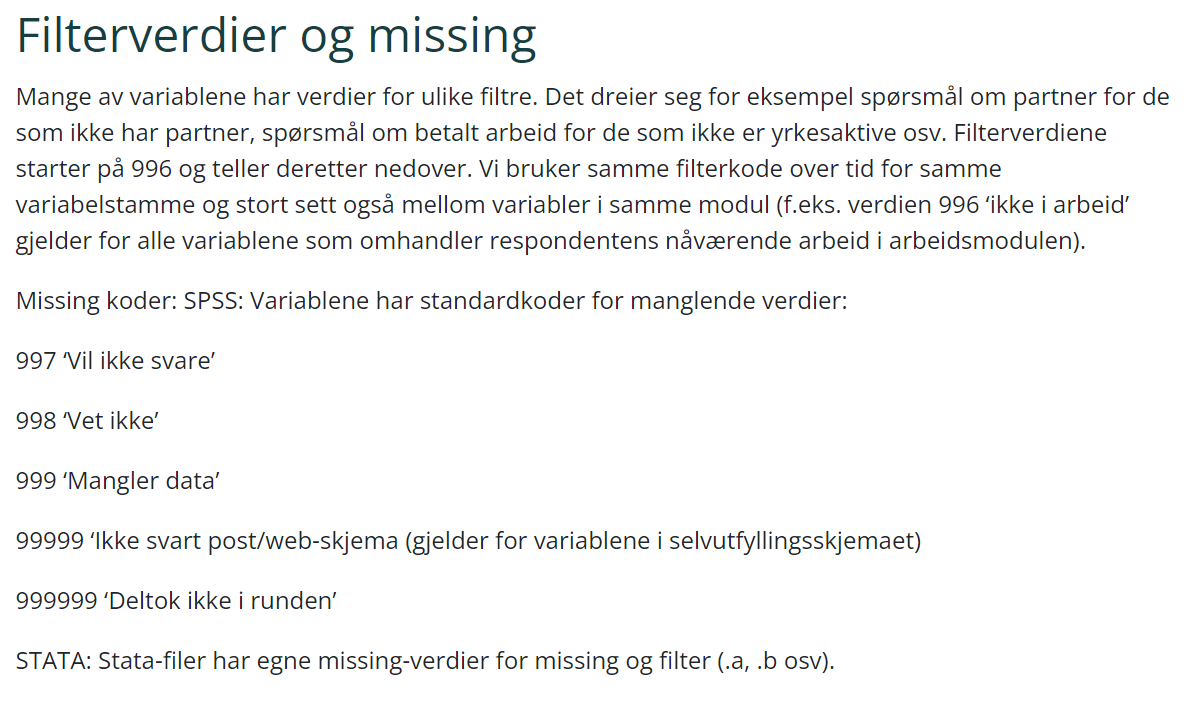
\includegraphics{./images/norlag_filterverdier.png}

}

\caption{Norlag missingverdier}

\end{figure}

Dette innebærer f.eks. at når man lager en frekvenstabell vil man få ut
frekvenstabell for både gyldige verdier og missingverdier, men
prosentuering vil bare være for de gyldige verdiene. Gitt at funksjonen
støtter dette formatet, vel å merke. Hvis dette ikke er kodet riktig i
datasettet vil missingverdiene kunne påvirke beregninger av gjennomsnitt
vesentlig.

\hypertarget{luxf8sning-fiks-alt-i-en-fei}{%
\section{Løsning: Fiks alt i en
fei}\label{luxf8sning-fiks-alt-i-en-fei}}

For å gjøre en lang historie kort, så trenger vi å fikse en del ting når
vi leser inn data fra formater som Stata og SPSS. Den etterfølgende
koden fikser følgende for \emph{hele} datasettet, og eksempelet er ved
bruk av NorLAG-dataene.

Her er det brukt Stata-formatet. Ovenfor sier dokumentasjonen av NorLAG
at Stata-formatet har egne missing-verdier som .a, .b osv. Pussig nok er
det datasettet som ble brukt her ikke slik, men inneholder de
missingverdiene som er spesifisert for SPSS. Slikt kan skje, og det er
ekstremt viktig at man sjekker datasettet for å se om slike ting er
akkurat slik som dokumentasjonen sier!

Så da viser eksempelet nedenfor hvordan vi håndterer med disse angitte
missing-verdiene. Det blir tilsvarende hvis andre verdier er brukt, så
det skulle ikke spille noen rolle.

\begin{Shaded}
\begin{Highlighting}[]
\NormalTok{norlag }\OtherTok{\textless{}{-}} \FunctionTok{read\_stata}\NormalTok{(}\StringTok{"data/norlag\_panel2022.dta"}\NormalTok{) }\SpecialCharTok{\%\textgreater{}\%} 
    \FunctionTok{mutate}\NormalTok{(}\FunctionTok{across}\NormalTok{( }\FunctionTok{where}\NormalTok{(is.labelled) ,  }\SpecialCharTok{\textasciitilde{}}\FunctionTok{replace}\NormalTok{(., }
\NormalTok{                                        . }\SpecialCharTok{\%in\%} \FunctionTok{c}\NormalTok{(}\DecValTok{997}\NormalTok{, }\DecValTok{998}\NormalTok{, }\DecValTok{999}\NormalTok{, }\DecValTok{99999}\NormalTok{, }\DecValTok{999999}\NormalTok{), }
                                        \ConstantTok{NA}\NormalTok{))) }\SpecialCharTok{\%\textgreater{}\%}
  \FunctionTok{drop\_unused\_value\_labels}\NormalTok{() }\SpecialCharTok{\%\textgreater{}\%} 
  \FunctionTok{unlabelled}\NormalTok{()}
\end{Highlighting}
\end{Shaded}

Koden ovenfor kan være litt vanskelig å tolke for den uerfarne, men her
er forklaringen med angitt hvilke linjer som gjør hva:

\begin{enumerate}
\def\labelenumi{\arabic{enumi})}
\tightlist
\item
  Lese inn data fra Stataformat (linje 1)
\item
  Gjøre om koder som indikerer spesielle missing-verdier til NA (linje
  2-4)
\item
  Fjerne de nå ubrukte label-nivåene (jf. forrige punkt) (linje 5)
\item
  Gjøre om alle labelled-variable til factor (linje 6)
\end{enumerate}

Et viktig moment her er at denne koden omkoder \emph{alle} variable i
datasettet. Det er også viktig å fjerne missing-verdier før man gjør om
til factor fordi hvis ikke blir missing-verdiene til egne factor-nivåer.
Missing-kodene brukes på både kontinuerlige og kategoriske variable, men
vi må stole på at dokumentasjonen stemmer og at disse verdiene brukes
konsekvent på alle variable uansett type (hvis ikke annet er angitt).

For de som ønsker (eller trenger) å vite mer vil logikken forklares i de
etterfølgende kapitlene. Resultatet er nå at du skal ha fått et datasett
der alle missing-verdier er omkodet til NA, og alle variable med
\emph{labler} (dvs. kategoriske variable) er omkodet til
factor-variable.

\hypertarget{detaljert-gjennomgang}{%
\section{Detaljert gjennomgang}\label{detaljert-gjennomgang}}

\hypertarget{innlesning-med-haven}{%
\subsection{Innlesning med \{haven\}}\label{innlesning-med-haven}}

Formatene Stata, SPSS og SAS er proprietære og man trenger i
utgangspunktet disse softwarene for å åpne datafilene (og betale dyr
lisens). For å lese inn i R kan man bruke pakken \{haven\} som
inneholder spesialiserte funksjoner for å lese inn disse formatene.
Funksjonen \texttt{read\_stata()} leser inn dataene på en måte som
bevarer særegenhetene fra Stata-formatet.

\begin{Shaded}
\begin{Highlighting}[]
\NormalTok{norlag }\OtherTok{\textless{}{-}} \FunctionTok{read\_stata}\NormalTok{(}\StringTok{"data/norlag\_panel2022.dta"}\NormalTok{, }\AttributeTok{encoding =} \StringTok{"utf8"}\NormalTok{) }
\end{Highlighting}
\end{Shaded}

Merk at objektet \texttt{norlag} vil være av typen \emph{tibble} og
variablene vil være \emph{labelled}. Med \texttt{glimpse()} og selektere
bare de 10 første variablene får vi følgende output:

\begin{Shaded}
\begin{Highlighting}[]
\FunctionTok{glimpse}\NormalTok{(norlag[,}\DecValTok{1}\SpecialCharTok{:}\DecValTok{10}\NormalTok{])}
\end{Highlighting}
\end{Shaded}

\begin{verbatim}
Rows: 33,084
Columns: 10
$ ref_nr        <dbl> 5, 5, 5, 10, 10, 10, 12, 12, 12, 15, 15, 15, 18, 18, 18,~
$ round         <dbl> 1, 2, 3, 1, 2, 3, 1, 2, 3, 1, 2, 3, 1, 2, 3, 1, 2, 3, 1,~
$ iointervjumnd <dbl+lbl>      5,     11, 999999,      5,      5,      5,     ~
$ iointervjuyr  <dbl+lbl>   2002,   2007, 999999,   2002,   2007,   2017,   20~
$ ioalder       <dbl+lbl>     68,     72, 999999,     44,     49,     59,     ~
$ iolandb       <dbl+lbl>      1,      1,      1,      1,      1,      1,     ~
$ iolandb3      <dbl+lbl>     NA,     NA, 999999,      1,      1,      1,     ~
$ iosvar        <dbl+lbl>      1,      1, 999999,      1,      1,      1,     ~
$ iofodselsyr   <dbl> 1934, 1934, 1934, 1957, 1957, 1957, 1955, 1955, 1955, 19~
$ iokjonn       <dbl+lbl> 1, 1, 1, 2, 2, 2, 2, 2, 2, 2, 2, 2, 1, 1, 1, 1, 1, 1~
\end{verbatim}

Merk at variabeltypene her er enten kontinuerlige,
\texttt{\textless{}dbl\textgreater{}}, eller kontinuerlige med labler,
\texttt{\textless{}dbl+lbl\textgreater{}}. Det er også verd å merke seg
at kategoriske variable som kjønn er kontinuerlig med labler. Også alder
er kontinuerlig med labler, men her er nok lablene knyttet til
missing-verdier siden alder her er tall.

Det kan være greit å vite at det er noen flere argumenter i
innlesningen. Noen ganger får man problemer med æøå, og da kan man
spesifisere tegnsetting med `encoding = ``utf8'' som gjort over. Men
oftest vil man ikke trenge akkurat det.

\hypertarget{omkode-variable-som-er-labelled}{%
\subsection{Omkode variable som er
labelled}\label{omkode-variable-som-er-labelled}}

Noen ganger vil vi omkode en variabel. Et eksempel er variabelen he104.
Her er innholdet i den variabelen.

\begin{Shaded}
\begin{Highlighting}[]
\NormalTok{memisc}\SpecialCharTok{::}\FunctionTok{codebook}\NormalTok{(norlag}\SpecialCharTok{$}\NormalTok{he104)}
\end{Highlighting}
\end{Shaded}

\begin{verbatim}
================================================================================

   norlag$he104 'Hvordan vil du beskrive din økonomiske situasjon nå'

--------------------------------------------------------------------------------

   Storage mode: double
   Measurement: undefined

   Values and labels                                           N Percent
                                                                        
        1 'Veldig romslig'                                  1425     4.3
        2 'Romslig'                                         8039    24.3
        3 'Må være forsiktig, men klarer meg'               5152    15.6
        4 'Problemer med å få pengene til å strekke til'     551     1.7
        5 'Svært vanskelig økonomisk situasjon'              164     0.5
      999 'Mangler data'                                     403     1.2
    99999 'Ikke svart post/web-skjema'                      5158    15.6
   999999 'Deltok ikke i runden'                           12192    36.9
\end{verbatim}

Legg merke til at de tre nederste verdiene egentlig er varianter av å
mangle data. Disse verdiene skal normalt ikke være med i en videre
analyse, men er ``missing''. Vi bør fortelle R at disse verdiene ikke
skal tas med videre ved å omkode til NA.

Følgende kode gjør en omkoding til NA. I eksempelet har jeg lagt inn
linjeskift for mutate() for å tydeliggjøre de ulike delene.

\begin{itemize}
\tightlist
\item
  Første linje lager en ny variabel he104b som skal inne en kopi av
  he104. Funksjonen \texttt{replace()} tar så utgangspunkt i variabelen
  he104, og de verdiene som ikke er angitt at skal byttes ut vil
  beholdes fra denne.\\
\item
  Andre linje sier at hvis variabelen he104 er en av verdiene 999,
  99999, eller 999999, så\ldots{}
\item
  sier tredje linje at da skal de få verdien NA i stedet.
\end{itemize}

\begin{Shaded}
\begin{Highlighting}[]
\NormalTok{norlag }\SpecialCharTok{\%\textgreater{}\%} 
  \FunctionTok{mutate}\NormalTok{(}\AttributeTok{he104b =} \FunctionTok{replace}\NormalTok{(he104, }
\NormalTok{                         he104 }\SpecialCharTok{\%in\%} \FunctionTok{c}\NormalTok{(}\DecValTok{999}\NormalTok{, }\DecValTok{99999}\NormalTok{, }\DecValTok{999999}\NormalTok{), }
                         \ConstantTok{NA}\NormalTok{)) }\SpecialCharTok{\%\textgreater{}\%}  
    \FunctionTok{select}\NormalTok{(he104b) }\SpecialCharTok{\%\textgreater{}\%} 
\NormalTok{  memisc}\SpecialCharTok{::}\FunctionTok{codebook}\NormalTok{()}
\end{Highlighting}
\end{Shaded}

\begin{verbatim}
================================================================================

   he104b 'Hvordan vil du beskrive din økonomiske situasjon nå'

--------------------------------------------------------------------------------

   Storage mode: double
   Measurement: undefined

   Values and labels                                           N Valid Total
                                                                            
        1   'Veldig romslig'                                1425   9.3   4.3
        2   'Romslig'                                       8039  52.4  24.3
        3   'Må være forsiktig, men klarer meg'             5152  33.6  15.6
        4   'Problemer med å få pengene til å strekke til'   551   3.6   1.7
        5   'Svært vanskelig økonomisk situasjon'            164   1.1   0.5
      999   'Mangler data'                                     0   0.0   0.0
    99999   'Ikke svart post/web-skjema'                       0   0.0   0.0
   999999   'Deltok ikke i runden'                             0   0.0   0.0
       NA M                                                17753        53.7
\end{verbatim}

Legg merke til at output nå har de omtalte verdiene 0 observasjoner, men
lablene finnes i variabelen likevel! Lablene eksisterer altså uavhengig
av verdiene i variabelen, men det har kommet en linje til med verdien
NA. Det er det det ble omkodet til. Nå trenger vi jo ikke de lablene vi
omkodet, så de kan fjernes helt. Funksjoen
\texttt{drop\_unused\_value\_labels()} gjør akkurat det det høres ut
som. Her er et eksempel:

\begin{Shaded}
\begin{Highlighting}[]
\NormalTok{norlag }\SpecialCharTok{\%\textgreater{}\%} 
  \FunctionTok{select}\NormalTok{(he104) }\SpecialCharTok{\%\textgreater{}\%} 
  \FunctionTok{mutate}\NormalTok{(}\AttributeTok{he104 =} \FunctionTok{replace}\NormalTok{(he104, }
\NormalTok{                         he104 }\SpecialCharTok{\%in\%} \FunctionTok{c}\NormalTok{(}\DecValTok{999}\NormalTok{, }\DecValTok{99999}\NormalTok{, }\DecValTok{999999}\NormalTok{), }
                         \ConstantTok{NA}\NormalTok{)) }\SpecialCharTok{\%\textgreater{}\%}  
  \FunctionTok{drop\_unused\_value\_labels}\NormalTok{() }\SpecialCharTok{\%\textgreater{}\%} 
\NormalTok{  memisc}\SpecialCharTok{::}\FunctionTok{codebook}\NormalTok{()}
\end{Highlighting}
\end{Shaded}

\begin{verbatim}
================================================================================

   he104 'Hvordan vil du beskrive din økonomiske situasjon nå'

--------------------------------------------------------------------------------

   Storage mode: double
   Measurement: undefined

   Values and labels                                       N Valid Total
                                                                        
    1   'Veldig romslig'                                1425   9.3   4.3
    2   'Romslig'                                       8039  52.4  24.3
    3   'Må være forsiktig, men klarer meg'             5152  33.6  15.6
    4   'Problemer med å få pengene til å strekke til'   551   3.6   1.7
    5   'Svært vanskelig økonomisk situasjon'            164   1.1   0.5
   NA M                                                17753        53.7
\end{verbatim}

\hypertarget{alternativ-legg-til-user-specified-na}{%
\subsection{Alternativ: legg til
user-specified-na}\label{alternativ-legg-til-user-specified-na}}

En alternativ fremgangsmåte er mer slik man ville gjort i annen software
ved at man definerer disse verdiene som ``missing'', dvs NA. Funksjonen
\texttt{set\_na\_values()} definerer hvilke verdier som skal regnes som
NA, men uten å endre lablene eller kode om på annen måte.

\begin{Shaded}
\begin{Highlighting}[]
\NormalTok{norlag }\SpecialCharTok{\%\textgreater{}\%} 
  \FunctionTok{select}\NormalTok{(he104) }\SpecialCharTok{\%\textgreater{}\%} 
  \FunctionTok{set\_na\_values}\NormalTok{(}\AttributeTok{he104 =} \FunctionTok{c}\NormalTok{(}\DecValTok{999}\NormalTok{, }\DecValTok{99999}\NormalTok{, }\DecValTok{999999}\NormalTok{) ) }\SpecialCharTok{\%\textgreater{}\%} 
\NormalTok{  memisc}\SpecialCharTok{::}\FunctionTok{codebook}\NormalTok{()}
\end{Highlighting}
\end{Shaded}

\begin{verbatim}
================================================================================

   he104 'Hvordan vil du beskrive din økonomiske situasjon nå'

--------------------------------------------------------------------------------

   Storage mode: double
   Measurement: undefined
   Missing values: 999, 99999, 999999

   Values and labels                                           N Valid Total
                                                                            
        1   'Veldig romslig'                                1425   9.3   4.3
        2   'Romslig'                                       8039  52.4  24.3
        3   'Må være forsiktig, men klarer meg'             5152  33.6  15.6
        4   'Problemer med å få pengene til å strekke til'   551   3.6   1.7
        5   'Svært vanskelig økonomisk situasjon'            164   1.1   0.5
      999 M 'Mangler data'                                   403         1.2
    99999 M 'Ikke svart post/web-skjema'                    5158        15.6
   999999 M 'Deltok ikke i runden'                         12192        36.9
\end{verbatim}

I output står det nå en ``M'' mellom verdien og labelen, som angir at
dette er ``Missing''. I frekvenstabellen er det nå i prosentueringen
skilt mellom \emph{Valid} og \emph{Total}, der missing altså ikke er
regnet med blant gyldige verdier.

Men det er ryddigst å fjerne disse missing-verdiene og sette de til NA.
Funksjonen \texttt{zap\_na()} gjør disse verdiene om til NA, altså
omkoder alle missingverdiene til NA. Som i forrige variant vil da
lablene fremdeles eksistere, men disse kan fjernes på samme måte med
\texttt{drop\_unused\_value\_labels()}.

\begin{Shaded}
\begin{Highlighting}[]
\NormalTok{norlag }\SpecialCharTok{\%\textgreater{}\%} 
  \FunctionTok{select}\NormalTok{(he104) }\SpecialCharTok{\%\textgreater{}\%} 
  \FunctionTok{set\_na\_values}\NormalTok{(}\AttributeTok{he104 =} \FunctionTok{c}\NormalTok{(}\DecValTok{999}\NormalTok{, }\DecValTok{99999}\NormalTok{, }\DecValTok{999999}\NormalTok{) ) }\SpecialCharTok{\%\textgreater{}\%} 
  \FunctionTok{zap\_missing}\NormalTok{() }\SpecialCharTok{\%\textgreater{}\%} 
  \FunctionTok{drop\_unused\_value\_labels}\NormalTok{() }\SpecialCharTok{\%\textgreater{}\%} 
\NormalTok{  memisc}\SpecialCharTok{::}\FunctionTok{codebook}\NormalTok{()}
\end{Highlighting}
\end{Shaded}

\begin{verbatim}
================================================================================

   he104 'Hvordan vil du beskrive din økonomiske situasjon nå'

--------------------------------------------------------------------------------

   Storage mode: double
   Measurement: undefined

   Values and labels                                       N Valid Total
                                                                        
    1   'Veldig romslig'                                1425   9.3   4.3
    2   'Romslig'                                       8039  52.4  24.3
    3   'Må være forsiktig, men klarer meg'             5152  33.6  15.6
    4   'Problemer med å få pengene til å strekke til'   551   3.6   1.7
    5   'Svært vanskelig økonomisk situasjon'            164   1.1   0.5
   NA M                                                17753        53.7
\end{verbatim}

\hypertarget{omkoding-av-andre-verdier}{%
\section{Omkoding av andre verdier}\label{omkoding-av-andre-verdier}}

Vi starter med å lagre de endringene som ble testet ut over, og lagrer
disse i et nytt datasett som kalles \emph{norlag2} som vi bruker videre
i eksemplene.

\begin{Shaded}
\begin{Highlighting}[]
\NormalTok{norlag2 }\OtherTok{\textless{}{-}}\NormalTok{ norlag }\SpecialCharTok{\%\textgreater{}\%} 
  \FunctionTok{select}\NormalTok{(he104) }\SpecialCharTok{\%\textgreater{}\%} 
  \FunctionTok{mutate}\NormalTok{(}\AttributeTok{he104 =} \FunctionTok{replace}\NormalTok{(he104, }
\NormalTok{                         he104 }\SpecialCharTok{\%in\%} \FunctionTok{c}\NormalTok{(}\DecValTok{999}\NormalTok{, }\DecValTok{99999}\NormalTok{, }\DecValTok{999999}\NormalTok{), }
                         \ConstantTok{NA}\NormalTok{)) }\SpecialCharTok{\%\textgreater{}\%}  
  \FunctionTok{drop\_unused\_value\_labels}\NormalTok{() }
\end{Highlighting}
\end{Shaded}

\hypertarget{konverter-variable-til-et-mer-ordinuxe6rt-r-format}{%
\section{Konverter variable til et mer ordinært
R-format}\label{konverter-variable-til-et-mer-ordinuxe6rt-r-format}}

Vi starter med å lagre en kopi av datasettet med endrede labler.

\begin{Shaded}
\begin{Highlighting}[]
\NormalTok{norlag3 }\OtherTok{\textless{}{-}}\NormalTok{ norlag2 }\SpecialCharTok{\%\textgreater{}\%} 
  \FunctionTok{mutate}\NormalTok{(}\AttributeTok{he104 =} \FunctionTok{recode}\NormalTok{(he104, }
                          \StringTok{\textasciigrave{}}\AttributeTok{1}\StringTok{\textasciigrave{}} \OtherTok{=} \DecValTok{2}\NormalTok{ ,}
                          \StringTok{\textasciigrave{}}\AttributeTok{5}\StringTok{\textasciigrave{}} \OtherTok{=} \DecValTok{4}\NormalTok{,}
                        \AttributeTok{.combine\_value\_labels =} \ConstantTok{TRUE}\NormalTok{) ) }\SpecialCharTok{\%\textgreater{}\%} 
  \FunctionTok{add\_value\_labels}\NormalTok{(}\AttributeTok{he104 =} \FunctionTok{c}\NormalTok{(}\StringTok{"Romslig/veldig romslig"} \OtherTok{=} \DecValTok{2}\NormalTok{, }
                             \StringTok{"Problemer/store problemer"} \OtherTok{=} \DecValTok{4}\NormalTok{))}
\end{Highlighting}
\end{Shaded}

Men hva skjer når vi skal lage en fin tabell? Vi prøver med
\{gtsummary\} og \texttt{tbl\_summary()}.

\begin{Shaded}
\begin{Highlighting}[]
\FunctionTok{library}\NormalTok{(gtsummary)}
\NormalTok{norlag3 }\SpecialCharTok{\%\textgreater{}\%} 
  \FunctionTok{tbl\_summary}\NormalTok{(}\AttributeTok{include =}\NormalTok{ he104)}
\end{Highlighting}
\end{Shaded}

\begin{longtable}[]{@{}lc@{}}
\toprule()
\textbf{Characteristic} & \textbf{N = 33,084} \\
\midrule()
\endhead
Hvordan vil du beskrive din økonomiske situasjon nå & \\
2 & 9,464 (62\%) \\
3 & 5,152 (34\%) \\
4 & 715 (4.7\%) \\
Unknown & 17,753 \\
\bottomrule()
\end{longtable}

Tabellen vises altså uten lablene! Noe av poenget med å ha labler var jo
å at det skal syens\ldots{} Siden mange funksjoner i R i utgangspunktet
ikke er laget for labler er det rett og slett ikke støttet.

Men vi kan gjøre om variabelen med \texttt{as\_factor()}. Gjør om
lablene til faktor-nivåer og så lage en tabell med den endrede
variabelen. (OBS! funskjonen \texttt{as\_factor()} gjør bare nesten det
samme. \texttt{as\_factor()} er laget bl.a. for å håndtere labler, mens
\texttt{as\_factor()} ikke gjør det).

\begin{Shaded}
\begin{Highlighting}[]
\NormalTok{norlag3 }\SpecialCharTok{\%\textgreater{}\%} 
  \FunctionTok{mutate}\NormalTok{(}\AttributeTok{he104 =} \FunctionTok{as\_factor}\NormalTok{(he104)) }\SpecialCharTok{\%\textgreater{}\%} 
\NormalTok{  gtsummary}\SpecialCharTok{::}\FunctionTok{tbl\_summary}\NormalTok{(}\AttributeTok{include =}\NormalTok{ he104)}
\end{Highlighting}
\end{Shaded}

\begin{longtable}[]{@{}lc@{}}
\toprule()
\textbf{Characteristic} & \textbf{N = 33,084} \\
\midrule()
\endhead
Hvordan vil du beskrive din økonomiske situasjon nå & \\
Romslig/veldig romslig & 9,464 (62\%) \\
Må være forsiktig, men klarer meg & 5,152 (34\%) \\
Problemer/store problemer & 715 (4.7\%) \\
Unknown & 17,753 \\
\bottomrule()
\end{longtable}

\hypertarget{hvordan-gjuxf8re-alt-i-en-fei-alle-variable-samtidig}{%
\section{Hvordan gjøre alt i en fei: alle variable
samtidig}\label{hvordan-gjuxf8re-alt-i-en-fei-alle-variable-samtidig}}

For NorLAG er det noen missingverdier som er definert på tvers av hele
datasettet. Se dokumentasjon her: https://norlag.nsd.no/filterverdier Å
gjøre de operasjonene vi gjorde over for hver enkelt av de over 400
variablene er utrolig arbeidskrevende og drit kjedelig. Så det gidder vi
ikke. Men å omkode alle variable i et helt datasett krever litt mer
avanserte operasjoner. Her bruker vi \texttt{across()} som angir at vi
skal gjøre samme operasjon på de nærere angitte variablene. Vi kan enten
gi en liste med variabelnavn, eller sette et krav om at variablene skal
være av en viss type, starte med visse bokstaver eller tegn osv. I
eksempelet nedenfor angir vi bare at variabelene skal være av typen
`labelled', noe de aller fleste er. Missing-verdiene i datasettet er jo
felles for alle variable, så da kan vi bruke replace() og sette disse
til NA. Her er et eksempel:

\begin{Shaded}
\begin{Highlighting}[]
\NormalTok{norlag4 }\OtherTok{\textless{}{-}}\NormalTok{ norlag }\SpecialCharTok{\%\textgreater{}\%} 
  \FunctionTok{mutate}\NormalTok{(}\FunctionTok{across}\NormalTok{( }\FunctionTok{where}\NormalTok{(is.labelled) ,  }\SpecialCharTok{\textasciitilde{}}\FunctionTok{replace}\NormalTok{(., }
\NormalTok{                                        . }\SpecialCharTok{\%in\%} \FunctionTok{c}\NormalTok{(}\DecValTok{997}\NormalTok{, }\DecValTok{998}\NormalTok{, }\DecValTok{999}\NormalTok{, }\DecValTok{99999}\NormalTok{, }\DecValTok{999999}\NormalTok{), }
                                        \ConstantTok{NA}\NormalTok{))) }\SpecialCharTok{\%\textgreater{}\%}  
  \FunctionTok{drop\_unused\_value\_labels}\NormalTok{()                                           }
\end{Highlighting}
\end{Shaded}

I mutate-setningen skjer følgende:

\begin{itemize}
\tightlist
\item
  \texttt{across()} sier at vi skal gjøre det samme for flere variable,
  spesifisert med \texttt{where(is.labelled)}.
\item
  for disse skal vi bruke \texttt{replace()}, angitt ved
  \texttt{\textasciitilde{}replace()}
\item
  inni parentesen angis . som hver av de variablene som er plukket ut i
  \texttt{across()}. Så for disse variablene skal det byttes ut verdier
\item
  neste linje starter med \texttt{.}, som igjen henviser til de samme
  variablen, og hvis de har en av de opplistede verdiene
\item
  i så fall får de ny verdi \texttt{NA}
\end{itemize}

Dermed er samtlige labelled-variable omkodet på denne måten i en fei.

Da kan vi lage en tabell på nytt. Her får vi samme problem med at
lablene ikke synes, men missing-verdiene er i hvetr fall ryddet opp i.

\begin{Shaded}
\begin{Highlighting}[]
\NormalTok{norlag4 }\SpecialCharTok{\%\textgreater{}\%} 
\NormalTok{  gtsummary}\SpecialCharTok{::}\FunctionTok{tbl\_summary}\NormalTok{(}\AttributeTok{include =}\NormalTok{ he104)}
\end{Highlighting}
\end{Shaded}

\begin{longtable}[]{@{}lc@{}}
\toprule()
\textbf{Characteristic} & \textbf{N = 33,084} \\
\midrule()
\endhead
Hvordan vil du beskrive din økonomiske situasjon nå & \\
1 & 1,425 (9.3\%) \\
2 & 8,039 (52\%) \\
3 & 5,152 (34\%) \\
4 & 551 (3.6\%) \\
5 & 164 (1.1\%) \\
Unknown & 17,753 \\
\bottomrule()
\end{longtable}

Vi kan selvfølgelig endre til factor som gjort over, men da får vi igjen
et problem med å gjøre det en variabel om gangen. Igjen: det gidder vi
ikke. I stedet bruker vi en enkel funksjon som fikser biffen for hele
datasettet, nemlig \texttt{unlabelled()}.

\begin{Shaded}
\begin{Highlighting}[]
\NormalTok{norlag4 }\SpecialCharTok{\%\textgreater{}\%} 
  \FunctionTok{unlabelled}\NormalTok{() }\SpecialCharTok{\%\textgreater{}\%} 
\NormalTok{  gtsummary}\SpecialCharTok{::}\FunctionTok{tbl\_summary}\NormalTok{(}\AttributeTok{include =}\NormalTok{ he104)}
\end{Highlighting}
\end{Shaded}

\begin{longtable}[]{@{}lc@{}}
\toprule()
\textbf{Characteristic} & \textbf{N = 33,084} \\
\midrule()
\endhead
Hvordan vil du beskrive din økonomiske situasjon nå & \\
Veldig romslig & 1,425 (9.3\%) \\
Romslig & 8,039 (52\%) \\
Må være forsiktig, men klarer meg & 5,152 (34\%) \\
Problemer med å få pengene til å strekke til & 551 (3.6\%) \\
Svært vanskelig økonomisk situasjon & 164 (1.1\%) \\
Unknown & 17,753 \\
\bottomrule()
\end{longtable}

OBS! Unlabelled endrer alle labelled-variablene. Det er ikke sikkert at
vi vil det. Spesielt gjelder det at det kan være andre labler knyttet
til variable som skal være kontinuerlige. Men: hvis man har gjort en god
opprydning i datasetet i forkant, med de omkodinger som trengs (det må
nok gjøres en for en variabel), så er dette ganske greit.

\bookmarksetup{startatroot}

\hypertarget{fuxe5-oversikt-over-datasettet}{%
\chapter{Få oversikt over
datasettet}\label{fuxe5-oversikt-over-datasettet}}

\begin{Shaded}
\begin{Highlighting}[]
\FunctionTok{library}\NormalTok{(tidyverse)}
\end{Highlighting}
\end{Shaded}

\begin{verbatim}
-- Attaching packages --------------------------------------- tidyverse 1.3.2 --
v ggplot2 3.4.0      v purrr   0.3.5 
v tibble  3.1.8      v dplyr   1.0.10
v tidyr   1.2.1      v stringr 1.4.1 
v readr   2.1.3      v forcats 0.5.2 
-- Conflicts ------------------------------------------ tidyverse_conflicts() --
x dplyr::filter() masks stats::filter()
x dplyr::lag()    masks stats::lag()
\end{verbatim}

\begin{Shaded}
\begin{Highlighting}[]
\FunctionTok{library}\NormalTok{(haven)}
\FunctionTok{library}\NormalTok{(labelled)}
\end{Highlighting}
\end{Shaded}

\begin{Shaded}
\begin{Highlighting}[]
\NormalTok{norlag }\OtherTok{\textless{}{-}} \FunctionTok{read\_stata}\NormalTok{(}\StringTok{"data/norlag\_panel2022.dta"}\NormalTok{)}
\end{Highlighting}
\end{Shaded}

Vi har nå et datasett i minnet og vi bør ta en titt på det. Nå er det
mange hundre variable i datasettet, så det er lite hensiktsmessig å
printe det til konsollen fordi det er rett og slett ikke plass. I
tidligere kurs skal dere ha lært å bruke funksjonen \texttt{glimpse()},
men også her blir det mest rotete fordi det er så mange variable.

En enkel løsning er å bare se på noen få variable om gangen. Med
klammeparentes kan vi angi hvilke radnummer og kolonnenummer vi ønsker
se på med følgende syntax: \texttt{datasett{[}rader,\ kolonner{]}} der
altså komma skiller mellom rader og kolonner. Følgende eksempel viser
hvordan man kan bruke \texttt{head()} for å vise de første
observasjonene i datasettet med bare de første 5 variablene (altså:
kollonne nr 1-5).

\begin{Shaded}
\begin{Highlighting}[]
\FunctionTok{head}\NormalTok{(norlag[, }\DecValTok{1}\SpecialCharTok{:}\DecValTok{5}\NormalTok{])}
\end{Highlighting}
\end{Shaded}

\begin{verbatim}
# A tibble: 6 x 5
  ref_nr round iointervjumnd                 iointervjuyr ioalder               
   <dbl> <dbl> <dbl+lbl>                     <dbl+lbl>    <dbl+lbl>             
1      5     1      5                          2002           68                
2      5     2     11                          2007           72                
3      5     3 999999 [Deltok ikke i runden] 999999       999999 [Deltok ikke i~
4     10     1      5                          2002           44                
5     10     2      5                          2007           49                
6     10     3      5                          2017           59                
\end{verbatim}

Legg merke til at under hvert variabelnavn står det en liten tekst,
f.eks. eller \textless S3: haven\_labelled\textgreater. Det kan også stå
andre ting. dbl betyr at det er en kontinuerlig variabel, mens
haven\_labelled betyr at det er labler til alle eller noe verdier i
variabelen.

En tilsvarende variant er å bruke \texttt{glimpse()} bare på et utvalg
variable på tilsvarende måte. Her er et eksempel, men der vi ser på de
10 første variablene.

\begin{Shaded}
\begin{Highlighting}[]
\FunctionTok{glimpse}\NormalTok{(norlag[, }\DecValTok{1}\SpecialCharTok{:}\DecValTok{20}\NormalTok{])}
\end{Highlighting}
\end{Shaded}

\begin{verbatim}
Rows: 33,084
Columns: 20
$ ref_nr          <dbl> 5, 5, 5, 10, 10, 10, 12, 12, 12, 15, 15, 15, 18, 18, 1~
$ round           <dbl> 1, 2, 3, 1, 2, 3, 1, 2, 3, 1, 2, 3, 1, 2, 3, 1, 2, 3, ~
$ iointervjumnd   <dbl+lbl>      5,     11, 999999,      5,      5,      5,   ~
$ iointervjuyr    <dbl+lbl>   2002,   2007, 999999,   2002,   2007,   2017,   ~
$ ioalder         <dbl+lbl>     68,     72, 999999,     44,     49,     59,   ~
$ iolandb         <dbl+lbl>      1,      1,      1,      1,      1,      1,   ~
$ iolandb3        <dbl+lbl>     NA,     NA, 999999,      1,      1,      1,   ~
$ iosvar          <dbl+lbl>      1,      1, 999999,      1,      1,      1,   ~
$ iofodselsyr     <dbl> 1934, 1934, 1934, 1957, 1957, 1957, 1955, 1955, 1955, ~
$ iokjonn         <dbl+lbl> 1, 1, 1, 2, 2, 2, 2, 2, 2, 2, 2, 2, 1, 1, 1, 1, 1,~
$ iopafyll        <dbl+lbl> 0, 0, 0, 0, 0, 0, 0, 0, 0, 0, 0, 0, 2, 2, 2, 0, 0,~
$ iodeltagelse    <dbl+lbl> 5, 5, 5, 1, 1, 1, 2, 2, 2, 5, 5, 5, 3, 3, 3, 4, 4,~
$ ionorlag1kohort <dbl+lbl> 1, 1, 1, 1, 1, 1, 1, 1, 1, 1, 1, 1, 0, 0, 0, 1, 1,~
$ iododyr         <dbl+lbl> 9996, 9996, 9996, 9996, 9996, 9996, 9996, 9996, 99~
$ ssIO_sivil      <dbl+lbl>  2,  2, NA,  4,  4,  4,  2, NA,  2,  4,  4, NA, NA~
$ hh001c          <dbl+lbl>      1,      1, 999999,      1,      1,      1,   ~
$ hh002           <dbl> 2, 2, 999999, 3, 2, 2, 2, 999999, 2, 1, 1, 999999, 999~
$ pa001c          <dbl+lbl>      1,      1, 999999,      0,      1,      1,   ~
$ pa002c          <dbl+lbl>     NA,      1, 999999,     NA,      2,      2,   ~
$ pa003           <dbl+lbl>     60,     66, 999999,    996,     57,     67,   ~
\end{verbatim}

I denne output'en er den første kollonnen altså variabelnavnene,
deretter er det en kollonne som viser hva slags type variabel det er, og
deretter de første observasjonene på hver variabel slik at man får et
inntrykk av hvordan det ser ut. \texttt{glimpse()} gir altså omtrent
samme informasjon som \texttt{head()}, men er nok mer hensiktsmessig
hvis mange variable.

For å se nærmere på en variabel går an å bruke funksjonen
\texttt{look\_for()}, som primært er en søke-funksjon, men det gir også
informasjon om variabelen.

\begin{Shaded}
\begin{Highlighting}[]
\FunctionTok{look\_for}\NormalTok{(norlag, }\StringTok{"iokjonn"}\NormalTok{)}
\end{Highlighting}
\end{Shaded}

\begin{verbatim}
 pos variable label     col_type values    
 10  iokjonn  IOs kjønn dbl+lbl  [1] Mann  
                                 [2] Kvinne
\end{verbatim}

I output fremgår det at dette er den 10'ende variabelen, inneholder
informasjonen ``IOs kjønn'', er av typen numerisk med tilhørende labler,
og verdiene er 1 = Mann og 2 = Kvinne.

Det går også an å bare få ut variabel-label med funksjonen
\texttt{var\_label()} slik:

\begin{Shaded}
\begin{Highlighting}[]
\FunctionTok{var\_label}\NormalTok{(norlag}\SpecialCharTok{$}\NormalTok{iokjonn)}
\end{Highlighting}
\end{Shaded}

\begin{verbatim}
[1] "IOs kjønn"
\end{verbatim}

For å se labels på \emph{verdiene} bruk \textbf{val\_labels()}.

\begin{Shaded}
\begin{Highlighting}[]
\FunctionTok{val\_labels}\NormalTok{(norlag}\SpecialCharTok{$}\NormalTok{iokjonn)}
\end{Highlighting}
\end{Shaded}

\begin{verbatim}
  Mann Kvinne 
     1      2 
\end{verbatim}

\hypertarget{alternativ-pakken-memisc-og-codebook}{%
\subsection{\texorpdfstring{Alternativ: pakken \{memisc\} og
\texttt{codebook()}}{Alternativ: pakken \{memisc\} og codebook()}}\label{alternativ-pakken-memisc-og-codebook}}

Man vil klare seg greit med det vi har vist ovenfor. Men det finnes
flere måter å gjøre det på. Pakken \{memisc\} inneholder en rekke
funksjoner for å håndtere surveydata, som vi ikke skal gå nærmere inn på
her. Men akkurat funksjonen \texttt{codebook()} gir litt mer informativt
output enn \texttt{look\_for()}.

For å bruke denne må du installere pakken først. I eksempelet nedenfor
er pakken ikke lastet med library(), men angitt pakken direkte med
\texttt{memisc::} først. Dette kan være nyttig hvis man ikke skal bruke
noen andre funksjoner fra denne pakken.

\begin{Shaded}
\begin{Highlighting}[]
\NormalTok{memisc}\SpecialCharTok{::}\FunctionTok{codebook}\NormalTok{(norlag}\SpecialCharTok{$}\NormalTok{iokjonn)}
\end{Highlighting}
\end{Shaded}

\begin{verbatim}
================================================================================

   norlag$iokjonn 'IOs kjønn'

--------------------------------------------------------------------------------

   Storage mode: double
   Measurement: undefined

   Values and labels       N Percent
                                    
   1 'Mann'            16197    49.0
   2 'Kvinne'          16887    51.0
\end{verbatim}

Poenget her er altså bare å få en penere output og litt deskriptiv
statistikk samtidig.

\hypertarget{suxf8ke-i-datasettet-etter-variable}{%
\section{Søke i datasettet etter
variable}\label{suxf8ke-i-datasettet-etter-variable}}

Alle datasett skal komme med en dokumentasjon som sier hva hver variabel
inneholder og hvilke verdier som finnes i hver variable, og hva de
betyr. Dette leveres gjerne som en separat fil, ganske ofte i pdf eller
html format. NSD/Sikt leverer dokumentasjonen for Norlag i html-format.
(Ideelt burde det vært i et enkelt maskinlesbart format egnet til å
bruke til omkoding og labler for de som ønsker det, men de har valgt en
annen løsning).

Du kan søke i dokumentasjonen på samme måte som i andre filer, men det
kan være litt knotete. Et godt alternativ er å søke direkte i
datasettet. Funksjonen \texttt{look\_for()} søker både i variabelnavn,
verdier og labler. Her er et eksempel for hvordan finne variabler som
inneholder ordet ``yrkesinntekt''. Du kan også søke på kortere eller
lengre tekststrenger. (Søker du f.eks. bare på ``innt'' eller ``yrke''
så får du opp langt flere variable, så du må kanskje prøve deg litt
frem).

\begin{Shaded}
\begin{Highlighting}[]
\FunctionTok{look\_for}\NormalTok{(norlag, }\StringTok{"Yrkesinntekt"}\NormalTok{)}
\end{Highlighting}
\end{Shaded}

\begin{verbatim}
 pos variable       label                   col_type values                 
 353 inwyrkinnt     Yrkesinntekter NorLAG ~ dbl+lbl  [-5000] Value <0 >-5000
                                                     [5000] Value >0 <5000  
                                                     [999999999] Mangler da~
 371 inpartwyrkinnt Partner: yrkesinntekte~ dbl+lbl  [99999996] Filter: IO ~
                                                     [99999999] Mangler data
                                                     [999999999] Deltok ikk~
\end{verbatim}

Det er to variable som inneholder teksten ``yrkesinntekt''. Den første
variabelen har posisjon 353 i datasettet og har variabelnavnet
inwyrkinnt. Den andre variabelen har posisjon 371 og har navnet
inpartwyrkinnt. Vi fokuserer på den første.

Merk at når labelen avsluttes med \textasciitilde{} (uttales ``tilde'')
indikerer det at teksten er avkortet i outputvinduet. Du får opp hele
teksten ved å bruke \texttt{val\_label()} slik:

\begin{Shaded}
\begin{Highlighting}[]
\FunctionTok{var\_label}\NormalTok{(norlag}\SpecialCharTok{$}\NormalTok{inwyrkinnt)}
\end{Highlighting}
\end{Shaded}

\begin{verbatim}
[1] "Yrkesinntekter NorLAG longitudinell"
\end{verbatim}

\bookmarksetup{startatroot}

\hypertarget{grafikk}{%
\chapter{Grafikk}\label{grafikk}}

\begin{Shaded}
\begin{Highlighting}[]
\FunctionTok{library}\NormalTok{(tidyverse)}
\end{Highlighting}
\end{Shaded}

\begin{verbatim}
-- Attaching packages --------------------------------------- tidyverse 1.3.2 --
v ggplot2 3.4.0      v purrr   0.3.5 
v tibble  3.1.8      v dplyr   1.0.10
v tidyr   1.2.1      v stringr 1.4.1 
v readr   2.1.3      v forcats 0.5.2 
-- Conflicts ------------------------------------------ tidyverse_conflicts() --
x dplyr::filter() masks stats::filter()
x dplyr::lag()    masks stats::lag()
\end{verbatim}

Les inn datasettet abu89.rds med følgende kommando:

\begin{Shaded}
\begin{Highlighting}[]
\NormalTok{abu89 }\OtherTok{\textless{}{-}} \FunctionTok{readRDS}\NormalTok{(}\StringTok{"data/abu89.rds"}\NormalTok{) }
\end{Highlighting}
\end{Shaded}

Lag et stolpediagram som viser antall menn og kvinner i datasettet med
følgende kommando:

\begin{Shaded}
\begin{Highlighting}[]
\FunctionTok{ggplot}\NormalTok{(abu89, }\FunctionTok{aes}\NormalTok{(}\AttributeTok{x=}\NormalTok{female))}\SpecialCharTok{+}
  \FunctionTok{geom\_bar}\NormalTok{()}
\end{Highlighting}
\end{Shaded}

\begin{figure}[H]

{\centering 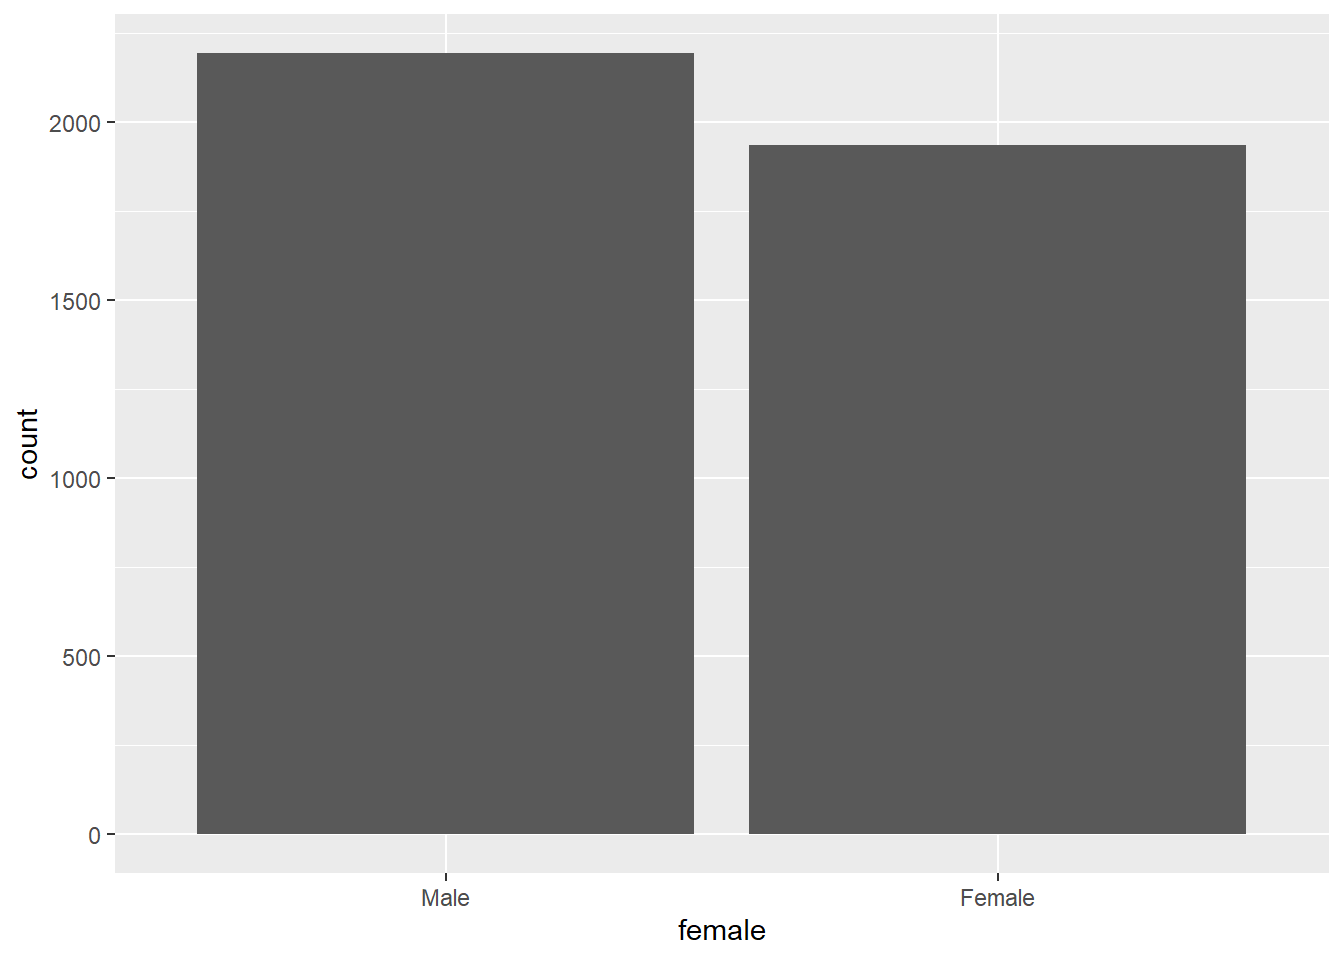
\includegraphics{./grafikk_files/figure-pdf/unnamed-chunk-3-1.pdf}

}

\end{figure}

For \texttt{geom\_bar()} bruker ggplot automatisk antall for y-aksen
hvis du ikke skriver noe annet. Merk at koden bare spesifiserer
x-variabelen. Da antar ggplot at du vil ha antall observasjoner som
høyde på stolpene. I det skjulte bruker ggplot en spesifikasjonen
\texttt{y\ =\ ..count..} som altså gir antallet.

\begin{enumerate}
\def\labelenumi{\arabic{enumi}.}
\setcounter{enumi}{9}
\item
  Lag plottet på nytt med andeler ved å spesifisere y som
  \texttt{..prop..} og sette \texttt{group\ =\ 1}.
  \texttt{aes(\ x\ =\ female,\ y\ =\ ..prop..,\ group\ =\ 1\ )}
\item
  Kanskje du heller vil ha prosent fremfor andeler? Prøv følgende:
  spesifiser y som \texttt{y\ =\ ..prop..*100} og så endre tekst på
  y-aksen med \texttt{labs()}. Altså multiplisere andelen med 100.
\end{enumerate}

For å lagre et plot til disk slik at du lett kan bruke det i f.eks. et
Word dokument bruker vi funksjonen ggsave(). Inni parentesen skriver du
filbanen der du vil lagre plottet, inkludert filhale for det formatet du
vil bruke. Det mest praktiske vil ofte være png-format, så da slutter
filnavnet på .png, så vil ggsave lagre i det formatet. Hvis du vil ha
plottet i pdf-format lar du tilsvarende filnavnet slutte på .pdf.\\
ggsave() lagrer det plottet som er i plotvinduet i Rstudio hvis du ikke
ber om noe annet. En bedre løsning er å legge hele plottet i et eget
objekt og så angi det objektet i ggsave(). Noe slikt:

\texttt{dittplot\ \textless{}-\ ggplot(…)\ +\ …\ \ ggsave(dittplot,\ filename\ =\ "output/dittfilnavn.png")}

\begin{enumerate}
\def\labelenumi{\arabic{enumi}.}
\setcounter{enumi}{11}
\item
  Lagre figuren til output-mappen i png-format med funksjonen ggsave()
  og gi filen et passende navn. For publisering kreves det ofte høy
  kvalitet på bildefilen, som spesifiseres med antall piksler angitt ved
  dpi. Forhåndsvalgt oppløsning for ggsave er dpi=300 som stort sett er
  tilstrekkelig. Hvis du trenger annen oppløsningen kan du spesifisere
  dpi høyere eller lavere.
\item
  Lag en høyoppløslig versjon ved å legge til dpi = 600 inni parentesen
  for ggsave() og gi filen et passende navn.
\item
  Lag en tilsvarende figur som i første oppgave, men nå for
  klassebakgrunn: Bruk samme kode, men bytt ut variabelen female med
  klasse89.
\end{enumerate}

I mange tilfeller vil dataene allerede være aggregert til en tabell. R
vil ikke vite forskjell på dette av seg selv. Da må du spesifisere at
y-variabelen er kolonnen med høyden på stolpen. Prøv med datasettet til
eksempel 3 til kapittel 1 i læreboka: music \textless-
read.csv(``data/chapter\_1/eg01-03music.csv'')

\begin{enumerate}
\def\labelenumi{\arabic{enumi}.}
\setcounter{enumi}{14}
\tightlist
\item
  Bruk ggplot som før, men med nye variabelnavn. For linjen med
  geom\_bar() må du nå spesifisere at ggplot ikke skal regne ut noe selv
  slik den ellers gjør. geom\_bar(stat = ``identity'')
\end{enumerate}

1.5 Histogram 16. Bruk datasettet abu89 og lag et histogram som viser
fordelingen av timelønn (time89). Tips: du må altså bytte ut
variabelnavn og bruke en annen geom\_*, nemlig geom\_histogram() 17.
Endre antall stolper ved å sette bins = og vurder om grover/fine
inndeling er best. 18. Gjør om histogrammet til å vise tetthet ved å
sette y = ..density.. 19. Legg til titler på aksene som du synes er
best. 20. Gjør egne vurderinger på endelig utseende på Når du er fornøyd
lagrer du plottet i output-mappen med et passende navn i png-format.

1.6 Boksplot 21. Lag et boksplot for timelønn. Endre da koden ved å
bruke geom\_boxplot() i stedet for geom\_histogram() som du brukte over.
Men sett nå time89 som y i stedet for x. 22. Boksplot er mest
interessant for å sammenligne grupper. Lag et boksplot for hver verdi av
klasse. Inni aes() setter du x = klasse89.

1.7 Tidsserieplot Noen data er tidsserier der vi ønsker å se utvikling
over tid. Et dagsaktuelt tema er overdødelighet i ulike land i på grunn
av Covid-pandemien. Prosjektet Human Mortality Database
(https://www.mortality.org/ ) har laget et datasett som heter Short-term
Mortality Fluctuations (STMF) som gir totale dødelighetsrater per uke
fra år 2000 og fremover for 38 land. (I skrivende stund tilgjengelig
frem til uke 43 i 2021). Et tilrettelagt datasett er lastet opp i Canvas
med filnavnet stmf\_prep.rds. Les inn datasettet med readRDS() og lagre
det i et objekt stmf. For mer informasjon om datasettet, se hjemmesiden.
Når man sammenligner total dødeligheten for land med tidligere år, så
vil vi kunne se om siste år har en overdødelighet sammenlignet med
disse. Datasettet inneholder tall for både totalt og for menn, kvinner,
og ulike aldersgrupper per land. Det kan være lurt å ikke plotte alt på
en gang. Lag først et plot for kun Norge siste to år. Bruk filter() til
å velge begge kjønn, kun Norge og siste to år, og lagre det som et nytt
objekt slik: nor \textless- stmf \%\textgreater\% filter(sex == ``b'',
age == ``Total'', country\_code == ``NOR'', year \textgreater= 2020)

Da kan du lage et linjediagram slik: ggplot(nor, aes(x = week, y =
rate\_total, col = as.factor(year))) + geom\_line()

Merk at fargen settes etter variabelen year, og den er satt som
as.factor() for å markere at det er kategorisk og ikke kontinuerlig
fargeskala. 23. Kan man si så mye om utviklingen? Hva bør man
sammenligne med? 24. Hvorfor tror du det kan være lurt å se på total
dødelighet fremfor døde direkte av Covid?

Juster koden over slik at du får med alle år for Norge og lag
linjediagrammet på nytt. I parentesen for aes() legger du til group =
year for å få en linje per år. Uten det blir det bare tull. Variabel
yr\_ind er en kategorisk variabel for å markere årene 2020 og 2021. I
aes() legger du også til color = yr\_ind for å si at det skal være
forskjellig farge etter denne indikatoren. Lag litt tykkere linjer ved å
spesifisere size = .9 inni parentesen for geom\_line(). Legg så til en
ny linje (sett + før linjeskift) i koden for å bestemme fargene manuelt
slik:\\
scale\_color\_manual(values = c(``gray70'', ``red'', ``blue''), labels =
c(``2000-2019'', ``2020'', ``2021'')) Du skal nå få et plot der alle
årene før 2020 er grå, mens 2020 og 2021 er henholdsvis rød og blå.
Argumentet labels = er til tegnforklaringen. 25. Hvordan har
dødeligheten vært totalt i Norge i 2020 og 2021 sammenlignet foregående
år? Kan du tenke deg noen grunner til dette resultatet? Nå kan du plotte
flere land og sammenligne utviklingen. For å se hvilke som er
tilgjengelige kjør følgende: unique(stmf\$country\_code) Juster koden du
brukte til å lage datasettet for kun Norge slik at du får med fire
valgfrie land. Du kan bruke \%in\% c(\ldots) for velge flere verdier på
landvariabelen. Her er et eksempel for å velge kun nordiske land:
filter(country\_code \%in\% c(``NOR'', ``SWE'', ``DNK'', ``FIN'')) Nå
kan du bruke samme kode for plottet, men legg til nederst (husk + før
linjeskift) følgende: facet\_wrap(\textasciitilde country\_code) Denne
koden gir et panel med et plot for hvert land slik at du lettere kan
sammenligne. Hvis det er stor forskjell på nivået kan du la y-skalaen
variere mellom landene ved å legge til scales = ``free'' inni parentesen
for facet\_wrap(). 26. Hvordan har dødeligheten vært i Norge under
pandemien sammenlignet med de andre landende du valgte? 27. Gjør
sammenligningen på nytt, men velg en annen aldersgruppe i stedet for
totalt. 28. Bruk det du har lært om labs() og theme\_*() til å gjøre
plottet penere og lagre i output-mappen. Du kan også flytte
tegnforklaringen ved å legge til følgende: theme(legend.position =
``top'')

\bookmarksetup{startatroot}

\hypertarget{deskriptive-tabeller}{%
\chapter{Deskriptive tabeller}\label{deskriptive-tabeller}}

\hypertarget{manuelle-tabeller-med-dplyr}{%
\section{Manuelle tabeller med
\{dplyr\}}\label{manuelle-tabeller-med-dplyr}}

Det er ofte mer effektivt å jobbe med

\hypertarget{pakken-gtsummary}{%
\section{Pakken \{gtsummary\}}\label{pakken-gtsummary}}

\hypertarget{pakken-datasummary}{%
\section{Pakken \{datasummary\}}\label{pakken-datasummary}}

\hypertarget{layout-med-gt}{%
\section{Layout med \{gt\}}\label{layout-med-gt}}

Pakken \{gt\} står for ``grammar of tables'' og er bygget opp som et
eget språk

\hypertarget{eksport-til-ms-word}{%
\section{Eksport til MS Word}\label{eksport-til-ms-word}}

Vi fokuserer her på eksport av resultater til tekstbehandlingsprogrammet
Word. Grunnen er at dette er det mest brukte. R er også svært godt egnet
til å eksportere til html, \(\LaTex\) og annet, men de som bruker slike
formater vil nok klare å finne ut av dette selv.

\bookmarksetup{startatroot}

\hypertarget{omkoding-av-factor-variable}{%
\chapter{Omkoding av
factor-variable}\label{omkoding-av-factor-variable}}

\begin{Shaded}
\begin{Highlighting}[]
\FunctionTok{library}\NormalTok{(haven)       }\CommentTok{\# Importere data fra SAS, SPSS og Stata}
\FunctionTok{library}\NormalTok{(tidyverse)   }\CommentTok{\# Pakker for generell datahåndtering og grafikk}
\FunctionTok{library}\NormalTok{(labelled)    }\CommentTok{\# Håndtering av variable med labler, importert fra annen software}
\FunctionTok{library}\NormalTok{(forcats)     }\CommentTok{\# Lettere omkoding av faktorvariable}
\end{Highlighting}
\end{Shaded}

\begin{Shaded}
\begin{Highlighting}[]
\NormalTok{norlag }\OtherTok{\textless{}{-}} \FunctionTok{read\_stata}\NormalTok{(}\StringTok{"data/norlag\_panel2022.dta"}\NormalTok{) }\SpecialCharTok{\%\textgreater{}\%} 
    \FunctionTok{mutate}\NormalTok{(}\FunctionTok{across}\NormalTok{( }\FunctionTok{where}\NormalTok{(is.labelled) ,  }\SpecialCharTok{\textasciitilde{}}\FunctionTok{replace}\NormalTok{(., }
\NormalTok{                                        . }\SpecialCharTok{\%in\%} \FunctionTok{c}\NormalTok{(}\DecValTok{997}\NormalTok{, }\DecValTok{998}\NormalTok{, }\DecValTok{999}\NormalTok{, }\DecValTok{99999}\NormalTok{, }\DecValTok{999999}\NormalTok{), }
                                        \ConstantTok{NA}\NormalTok{))) }\SpecialCharTok{\%\textgreater{}\%}
  \CommentTok{\# For hele datasettet fjernes ikke{-}brukte labler }
  \FunctionTok{drop\_unused\_value\_labels}\NormalTok{() }\SpecialCharTok{\%\textgreater{}\%} 
  \CommentTok{\# Så gjør alle variable om til mer ordinære R{-}format. Dvs. gjøre labler om til factor}
  \FunctionTok{unlabelled}\NormalTok{()}
\end{Highlighting}
\end{Shaded}

\hypertarget{factorvariable-med-skikkelig-lang-tekst}{%
\section{Factorvariable med skikkelig lang
tekst}\label{factorvariable-med-skikkelig-lang-tekst}}

Noen ganger har man et datasett som allerede er omgjort med
factor-variable. Eller du har en eller annen grunn til å ikke gå tilbake
til et tidligere steg for å omkode. Men du har factor-levels med
skikkelig lang tekst kan det være noe drit å kode om. Kan man gjøre
dette på en lurere måte? Minst mulig tårer? Ja, selvsagt.

I NorLAG er variabelen wr117zz svar på et spørsmål om ``Mulighet for å
redusert arbeidstid (deltid)''. Når denne variabelen er gjort om til
factor kan man se hvilke verdier variabelen har med bruke av funksjonen
\emph{levels()} slik:

\begin{Shaded}
\begin{Highlighting}[]
\FunctionTok{levels}\NormalTok{(norlag}\SpecialCharTok{$}\NormalTok{wr117zz)}
\end{Highlighting}
\end{Shaded}

\begin{verbatim}
[1] "Nei"                                                               
[2] "Ja"                                                                
[3] "filter: jobber deltid"                                             
[4] "filter: selvstendig næringsdrivende (NorLAG3 inkl frilanser/annet)"
[5] "filter: ikke i arbeid"                                             
\end{verbatim}

\begin{Shaded}
\begin{Highlighting}[]
\FunctionTok{table}\NormalTok{(norlag}\SpecialCharTok{$}\NormalTok{wr117zz)}
\end{Highlighting}
\end{Shaded}

\begin{verbatim}

                                                               Nei 
                                                              1360 
                                                                Ja 
                                                              4146 
                                             filter: jobber deltid 
                                                              1964 
filter: selvstendig næringsdrivende (NorLAG3 inkl frilanser/annet) 
                                                              1171 
                                             filter: ikke i arbeid 
                                                              6238 
\end{verbatim}

La oss si at vi vil kode om slik at vi får en variabel som bare er om
vedkommende har mulighet til å jobbe deltid eller ikke. De som allerede
jobber deltid har jo åpenbart mulighet til det, så de skal kodes om til
``Ja''. De andre kategoriene er egentlig grunner til at det mangler
data, så de skal settes til NA. En mulighet er da å omkode som følger:

\begin{Shaded}
\begin{Highlighting}[]
\NormalTok{norlag\_omkodet }\OtherTok{\textless{}{-}}\NormalTok{ norlag }\SpecialCharTok{\%\textgreater{}\%}
  \FunctionTok{mutate}\NormalTok{(}\AttributeTok{redarbtid =} \FunctionTok{replace}\NormalTok{(wr117zz, wr117zz }\SpecialCharTok{==} \StringTok{"filter: jobber deltid"}\NormalTok{, }\StringTok{"Ja"}\NormalTok{), }
         \AttributeTok{redarbtid =} \FunctionTok{replace}\NormalTok{(redarbtid, redarbtid }\SpecialCharTok{==} \StringTok{"filter: selvstendig næringsdrivende (NorLAG3 inkl frilanser/annet)"}\NormalTok{, }\ConstantTok{NA}\NormalTok{), }
         \AttributeTok{redarbtid =} \FunctionTok{replace}\NormalTok{(redarbtid, redarbtid }\SpecialCharTok{==} \StringTok{"filter: ikke i arbeid"}\NormalTok{, }\ConstantTok{NA}\NormalTok{), }
         \AttributeTok{redarbtid =} \FunctionTok{replace}\NormalTok{(redarbtid, redarbtid }\SpecialCharTok{==} \StringTok{"vil ikke svare"}\NormalTok{, }\ConstantTok{NA}\NormalTok{),}
         \AttributeTok{redarbtid =} \FunctionTok{replace}\NormalTok{(redarbtid, redarbtid }\SpecialCharTok{==} \StringTok{"vet ikke"}\NormalTok{, }\ConstantTok{NA}\NormalTok{),}
         \AttributeTok{redarbtid =} \FunctionTok{replace}\NormalTok{(redarbtid, redarbtid }\SpecialCharTok{==} \StringTok{"mangler data"}\NormalTok{, }\ConstantTok{NA}\NormalTok{),}
         \AttributeTok{redarbtid =} \FunctionTok{replace}\NormalTok{(redarbtid, redarbtid }\SpecialCharTok{==} \StringTok{"Deltok ikke i runden"}\NormalTok{, }\ConstantTok{NA}\NormalTok{)) }\SpecialCharTok{\%\textgreater{}\%} 
  \FunctionTok{droplevels}\NormalTok{()}
\end{Highlighting}
\end{Shaded}

Dette funker, men blir ganske mye tekst å skrive, og da kan man også
lett gjøre skrivefeil. Husk at faktornivåene må angis helt nøyaktig slik
de er skrevet! Merk at den siste funksjone, \emph{droplevels()}, bare
fjerner faktor-levels som ikke er i bruk.

I output for faktor-levels angir klammeparentesen gir rekkefølgen på
disse verdiene. Vi kan bruke denne informasjonen direkte i omkodingen
for å unngå å skrive så veldig mye. Når man bruker levels() får man en
liten vektor med verdier, og disse kan man altså henvise til med
rekkefølgen. Her er et eksempel for bare å bytte ut de som jobber deltid
til ``Ja'':

\begin{Shaded}
\begin{Highlighting}[]
\NormalTok{norlag\_omkodet }\OtherTok{\textless{}{-}}\NormalTok{ norlag }\SpecialCharTok{\%\textgreater{}\%}
  \FunctionTok{mutate}\NormalTok{(}\AttributeTok{redarbtid =} \FunctionTok{replace}\NormalTok{(wr117zz, wr117zz }\SpecialCharTok{==} \FunctionTok{levels}\NormalTok{(wr117zz)[}\DecValTok{3}\NormalTok{], }\StringTok{"Ja"}\NormalTok{)) }\SpecialCharTok{\%\textgreater{}\%} 
  \FunctionTok{droplevels}\NormalTok{()}
\end{Highlighting}
\end{Shaded}

Trikset her er altså å bruke levels() og vise til hvilket nummer i
rekkefølgen. Da unngår vi også faren for skrivefeil.

Vi vil også kode om alle de andre verdiene, nummer 4-9 til NA. Det kan
vi gjøre på samme måte, men vi behøver ikke skrive en ny linje for hver
verdi. Den logiske operatoren == kan man bruke når man skal sjekke om to
verdier er like. Hvis vi skal se om en verdi er lik en av flere mulige
kan vi bruke \%in\% og så en liste med verdier. levels() gir en liste
med verdier, så da kan vi angi den direkte og alle verdiene 4 til 9 ved
å skrive 4:9. Samlet blir det da slik:

\begin{Shaded}
\begin{Highlighting}[]
\NormalTok{norlag\_omkodet }\OtherTok{\textless{}{-}}\NormalTok{ norlag }\SpecialCharTok{\%\textgreater{}\%}
  \FunctionTok{mutate}\NormalTok{(}\AttributeTok{redarbtid =} \FunctionTok{replace}\NormalTok{(wr117zz, wr117zz }\SpecialCharTok{==} \FunctionTok{levels}\NormalTok{(wr117zz)[}\DecValTok{3}\NormalTok{], }\StringTok{"Ja"}\NormalTok{), }
         \AttributeTok{redarbtid =} \FunctionTok{replace}\NormalTok{(redarbtid, redarbtid }\SpecialCharTok{\%in\%} \FunctionTok{levels}\NormalTok{(wr117zz)[}\DecValTok{4}\SpecialCharTok{:}\DecValTok{9}\NormalTok{], }\ConstantTok{NA}\NormalTok{)) }\SpecialCharTok{\%\textgreater{}\%} 
  \FunctionTok{droplevels}\NormalTok{()}

\NormalTok{memisc}\SpecialCharTok{::}\FunctionTok{codebook}\NormalTok{(norlag\_omkodet}\SpecialCharTok{$}\NormalTok{redarbtid)}
\end{Highlighting}
\end{Shaded}

\begin{verbatim}
================================================================================

   norlag_omkodet$redarbtid

--------------------------------------------------------------------------------

   Storage mode: integer
   Factor with 2 levels

   Levels and labels     N Valid Total
                                      
    1 'Nei'           1360  18.2   4.1
    2 'Ja'            6110  81.8  18.5
   NA                25614        77.4
\end{verbatim}

\appendix
\addcontentsline{toc}{part}{Appendices}

\hypertarget{omkoding-av-labelled-variable-i-innlesning-fra-stata}{%
\chapter{Omkoding av labelled-variable i innlesning fra
Stata}\label{omkoding-av-labelled-variable-i-innlesning-fra-stata}}

I tillegg skal vi bruke pakker for generell datahåndtering som er samlet
i pakken \{tidyverse\}, deriblant en pakke \{forcats\} for håndtering av
kategoriske variable.

\begin{Shaded}
\begin{Highlighting}[]
\FunctionTok{library}\NormalTok{(tidyverse)   }\CommentTok{\# Generelle funksjoner for datahåndtering}
\FunctionTok{library}\NormalTok{(forcats)     }\CommentTok{\# Funksjoner spesielt for factor{-}variable}
\end{Highlighting}
\end{Shaded}

I dette kapittelet skal vi bruke følgende pakker:

\begin{Shaded}
\begin{Highlighting}[]
\FunctionTok{library}\NormalTok{(haven)       }\CommentTok{\# Importere data fra SAS, SPSS og Stata}
\FunctionTok{library}\NormalTok{(tidyverse)   }\CommentTok{\# Pakker for generell datahåndtering og grafikk}
\FunctionTok{library}\NormalTok{(labelled)    }\CommentTok{\# Håndtering av variable med labler, importert fra annen software}
\FunctionTok{library}\NormalTok{(forcats)     }\CommentTok{\# Lettere omkoding av faktorvariable}
\end{Highlighting}
\end{Shaded}

Det er fult mulig å jobbe med data som inneholder labler og gjøre
omkodinger basert på dette. Omkoding av variable avhenger av hva slags
type variable det er, så man må gjøre det på en litt annen måte når det
er snakk om labler.

Mitt anbefaling vil da være å gjøre all omkoding tidlig i scriptet

Når man leser inn data som inkluderer labler kan man velge å omkode
disse med en gang før man gjør om til factor-variable.

I så fall kan det gjøres etter mønster som i følgende kode. Eller man
kan vente til man har gjort om til factor-variable som forklares noe
senere i dette dokumentet.

\begin{Shaded}
\begin{Highlighting}[]
\NormalTok{norlag }\OtherTok{\textless{}{-}} \FunctionTok{read\_stata}\NormalTok{(}\StringTok{"data/norlag\_panel2022.dta"}\NormalTok{) }\SpecialCharTok{\%\textgreater{}\%} 
    \FunctionTok{mutate}\NormalTok{(}\FunctionTok{across}\NormalTok{( }\FunctionTok{where}\NormalTok{(is.labelled) ,  }\SpecialCharTok{\textasciitilde{}}\FunctionTok{replace}\NormalTok{(., }
\NormalTok{                                        . }\SpecialCharTok{\%in\%} \FunctionTok{c}\NormalTok{(}\DecValTok{997}\NormalTok{, }\DecValTok{998}\NormalTok{, }\DecValTok{999}\NormalTok{, }\DecValTok{99999}\NormalTok{, }\DecValTok{999999}\NormalTok{), }
                                        \ConstantTok{NA}\NormalTok{))) }\SpecialCharTok{\%\textgreater{}\%}
  \CommentTok{\# For hele datasettet fjernes ikke{-}brukte labler }
  \FunctionTok{drop\_unused\_value\_labels}\NormalTok{()  }
\end{Highlighting}
\end{Shaded}

Så kan du gjøre andre analyser etter dette. Hvis du trenger å gå tilbake
for å omkode flere labelled-variable, så legges dette til i
mutate-setningen over. Det er lurt å gjøre all den typen omkoding ett
sted, slik at du får et datasett som er ferdig ryddet og klart til andre
analyser.

La oss si at vi det er mindre viktig om man har det romslig eller veldig
romslig. Det er heller ikke så viktig å skille mellom de som `problemer'
og de som har det `svært vanskelig'. Da ønsker vi å slå sammen disse
kategoriene.

For å omkode en variabel som har labler kan vi bruke \texttt{recode()}.
Det gjør vi typisk innenfor en mutate-setning.

\begin{itemize}
\tightlist
\item
  Første linje sier at det skal lages en ny variabel, som er en rekodet
  variant av he104
\item
  Andre linje sier at alle med verdien 1 skal gjøres om til verdien 2
\item
  Tredje linje sier at alle med verdien 5 skal gjøres om til verdien 4
\end{itemize}

Legg merke til at den opprinneligve verdien angis innenfor apostrof
\texttt{1}, mens den nye verdien ikke skal angis med apostrof.

\begin{Shaded}
\begin{Highlighting}[]
\NormalTok{norlag }\SpecialCharTok{\%\textgreater{}\%} 
  \FunctionTok{mutate}\NormalTok{(}\AttributeTok{okonomi =} \FunctionTok{recode}\NormalTok{(he104, }
                          \StringTok{\textasciigrave{}}\AttributeTok{1}\StringTok{\textasciigrave{}} \OtherTok{=} \DecValTok{2}\NormalTok{ ,}
                          \StringTok{\textasciigrave{}}\AttributeTok{5}\StringTok{\textasciigrave{}} \OtherTok{=} \DecValTok{4}\NormalTok{) ) }\SpecialCharTok{\%\textgreater{}\%} 
  \FunctionTok{select}\NormalTok{(okonomi) }\SpecialCharTok{\%\textgreater{}\%} 
\NormalTok{  memisc}\SpecialCharTok{::}\FunctionTok{codebook}\NormalTok{()}
\end{Highlighting}
\end{Shaded}

\begin{verbatim}
================================================================================

   okonomi 'Hvordan vil du beskrive din økonomiske situasjon nå'

--------------------------------------------------------------------------------

   Storage mode: double
   Measurement: undefined

   Values and labels                                       N Valid Total
                                                                        
    1   'Veldig romslig'                                   0   0.0   0.0
    2   'Romslig'                                       9464  61.7  28.6
    3   'Må være forsiktig, men klarer meg'             5152  33.6  15.6
    4   'Problemer med å få pengene til å strekke til'   715   4.7   2.2
    5   'Svært vanskelig økonomisk situasjon'              0   0.0   0.0
   NA M                                                17753        53.7
\end{verbatim}

Legg merke til at de opprinnelge lablene fremdeles er der, men to av
kategoriene har nå null observasjoner. Det innebærer jo også at lablene
er litt misvisende, for det er jo egentlig kombinasjoner.

Å omkode lablene kan også gjøres. Funksjonen \emph{add\_value\_labels()}
angir hvilken variabel lablene skal angis for, og så settes ny label og
hvilken verdi det tilsvarer. Lablene for verdier som ikke er nevnt blir
beholdt slik de er.

\begin{Shaded}
\begin{Highlighting}[]
\NormalTok{norlag }\SpecialCharTok{\%\textgreater{}\%} 
  \FunctionTok{mutate}\NormalTok{(}\AttributeTok{he104 =} \FunctionTok{recode}\NormalTok{(he104, }
                          \StringTok{\textasciigrave{}}\AttributeTok{1}\StringTok{\textasciigrave{}} \OtherTok{=} \DecValTok{2}\NormalTok{ ,}
                          \StringTok{\textasciigrave{}}\AttributeTok{5}\StringTok{\textasciigrave{}} \OtherTok{=} \DecValTok{4}\NormalTok{,}
                        \AttributeTok{.combine\_value\_labels =} \ConstantTok{TRUE}\NormalTok{) ) }\SpecialCharTok{\%\textgreater{}\%} 
  \FunctionTok{select}\NormalTok{(he104) }\SpecialCharTok{\%\textgreater{}\%} 
  \FunctionTok{add\_value\_labels}\NormalTok{(}\AttributeTok{he104 =} \FunctionTok{c}\NormalTok{(}\StringTok{"Romslig/veldig romslig"} \OtherTok{=} \DecValTok{2}\NormalTok{, }
                             \StringTok{"Problemer/store problemer"} \OtherTok{=} \DecValTok{4}\NormalTok{)) }\SpecialCharTok{\%\textgreater{}\%} 
\NormalTok{  memisc}\SpecialCharTok{::}\FunctionTok{codebook}\NormalTok{()}
\end{Highlighting}
\end{Shaded}

\begin{verbatim}
================================================================================

   he104 'Hvordan vil du beskrive din økonomiske situasjon nå'

--------------------------------------------------------------------------------

   Storage mode: double
   Measurement: undefined

   Values and labels                            N Valid Total
                                                             
    2   'Romslig/veldig romslig'             9464  61.7  28.6
    3   'Må være forsiktig, men klarer meg'  5152  33.6  15.6
    4   'Problemer/store problemer'           715   4.7   2.2
   NA M                                     17753        53.7
\end{verbatim}



\end{document}
